% This is the Reed College LaTeX thesis template. Most of the work
% for the document class was done by Sam Noble (SN), as well as this
% template. Later comments etc. by Ben Salzberg (BTS). Additional
% restructuring and APA support by Jess Youngberg (JY).
% Your comments and suggestions are more than welcome; please email
% them to cus@reed.edu
%
% See https://www.reed.edu/cis/help/LaTeX/index.html for help. There are a
% great bunch of help pages there, with notes on
% getting started, bibtex, etc. Go there and read it if you're not
% already familiar with LaTeX.
%
% Any line that starts with a percent symbol is a comment.
% They won't show up in the document, and are useful for notes
% to yourself and explaining commands.
% Commenting also removes a line from the document;
% very handy for troubleshooting problems. -BTS

% As far as I know, this follows the requirements laid out in
% the 2002-2003 Senior Handbook. Ask a librarian to check the
% document before binding. -SN

%%
%% Preamble
%%
% \documentclass{<something>} must begin each LaTeX document
\documentclass[12pt,twoside]{templates/facsothesis}
 \renewcommand{\familydefault}{\sfdefault}
% Packages are extensions to the basic LaTeX functions. Whatever you
% want to typeset, there is probably a package out there for it.
% Chemistry (chemtex), screenplays, you name it.
% Check out CTAN to see: https://www.ctan.org/
%%
\ifxetex
  \usepackage{polyglossia}
  \setmainlanguage{spanish}
  % Tabla en lugar de cuadro
  \gappto\captionsspanish{\renewcommand{\tablename}{Tabla}
          \renewcommand{\listtablename}{Índice de tablas}}
\else
  \usepackage[spanish,es-tabla]{babel}
\fi
%\usepackage[spanish]{babel}
\usepackage{graphicx,latexsym}
\usepackage{amsmath}
\usepackage{amssymb,amsthm}
\usepackage{longtable,booktabs,setspace}
\usepackage{chemarr} %% Useful for one reaction arrow, useless if you're not a chem major
\usepackage[hyphens]{url}
% Added by CII
%\usepackage{hyperref}
\usepackage[colorlinks = true,
            linkcolor = blue,
            urlcolor  = blue,
            citecolor = blue,
            anchorcolor = blue]{hyperref}
\usepackage{titlesec}
\titleformat{\chapter}[display]{\normalfont\bfseries}{}{0pt}{\Huge}
\titlespacing*{\chapter}{0pt}{-50pt}{12pt}
\usepackage{float}
\floatplacement{figure}{H}
% End of CII addition
\usepackage{rotating}
\usepackage{placeins} % para fijar la posición de las tablas con \FloatBarrier
\usepackage{helvet}

\usepackage[]{natbib}


% Next line commented out by CII
%\usepackage{biblatex}
%\usepackage{natbib}
% Comment out the natbib line above and uncomment the following two lines to use the new
% biblatex-chicago style, for Chicago A. Also make some changes at the end where the
% bibliography is included.
%\usepackage{biblatex-chicago}
%\bibliography{thesis}


% Added by CII (Thanks, Hadley!)
% Use ref for internal links
\renewcommand{\hyperref}[2][???]{\autoref{#1}}
\def\chapterautorefname{Chapter}
\def\sectionautorefname{Section}
\def\subsectionautorefname{Subsection}
% End of CII addition

% Added by CII
\usepackage{caption}
\captionsetup{width=5in}
% End of CII addition

% \usepackage{times} % other fonts are available like times, bookman, charter, palatino

% Syntax highlighting #22

% To pass between YAML and LaTeX the dollar signs are added by CII
\title{PERFILES DE INDIVIDUALISMO Y SU RELACIÓN CON EL APOYO A LA DEMOCRACIA DELEGATIVA EN LA SOCIEDAD CHILENA}
\author{GABRIEL CORTÉS PAREDES}
% The month and year that you submit your FINAL draft TO THE LIBRARY (May or December)
\date{Santiago de Chile, 2023}
\division{}
\advisor{Profesora guía: Macarena Orchard}
\institution{FACULTAD DE CIENCIAS SOCIALES E HISTORIA}
\degree{Tesis para optar al grado de magíster en Métodos para la Investigación Social}
%If you have two advisors for some reason, you can use the following
% Uncommented out by CII
% End of CII addition

%%% Remember to use the correct department!
\department{}
% if you're writing a thesis in an interdisciplinary major,
% uncomment the line below and change the text as appropriate.
% check the Senior Handbook if unsure.
%\thedivisionof{The Established Interdisciplinary Committee for}
% if you want the approval page to say "Approved for the Committee",
% uncomment the next line
%\approvedforthe{Committee}

% Added by CII
%%% Copied from knitr
%% maxwidth is the original width if it's less than linewidth
%% otherwise use linewidth (to make sure the graphics do not exceed the margin)
\makeatletter
\def\maxwidth{ %
  \ifdim\Gin@nat@width>\linewidth
    \linewidth
  \else
    \Gin@nat@width
  \fi
}
\makeatother

%Added by @MyKo101, code provided by @GerbrichFerdinands

\setlength\parindent{0pt}


% Added by CII

\providecommand{\tightlist}{%
  \setlength{\itemsep}{0pt}\setlength{\parskip}{0pt}}



\Dedication{

}

\Preface{
\emph{``If success and failure are the result of individual effort, those at the top can hardly be blamed -- unless, of course, they are politician''} (Bellah et al, 1996, p.xv)
}

\Acknowledgements{
No puedo comenzar este documento, que representa el cierre de una etapa significativa en mi vida personal y profesional, sin antes expresar mi profundo agradecimiento a mi familia por el apoyo incondicional brindado en estos últimos años. Espero poder retribuir, aunque sea en parte, todo lo que han hecho por mí.

También debo agradecer a todas las personas que dedicaron su tiempo, consejo y reflexión a esta tesis. Agradezco a la profesora Macarena Orchard, cuya dedicación y compromiso fueron fundamentales para pulir este trabajo y profundizar cada reflexión. Al profesor Cristóbal Moya, por su invaluable guía metodológica. Igualmente, agradezco al profesor Raimundo Frei, a Camila Joustra y a todos mis compañer-s del curso de Seminario, quienes me acompañaron en este proceso a lo largo del año. Todos ustedes no solo hicieron posible esta investigación, sino que la enriquecieron enormemente.

Por último, es mi deber agradecer a Subdirección de Capital Humano de ANID (y a quienes me apoyaron en mi postulación, especialmente a la profesora Catalina Arteaga y al profesor Patricio Saavedra) por su contribución al financiamiento de mis estudios de posgrado a través de la Beca Magíster Nacional (2022-22221874).

¡Muchas gracias!
}

\Abstract{
Esta investigación buscó explorar las consecuencias políticas, sociales y económicas derivadas de la relación entre el individualismo y las preferencias políticas. En concretó, se propuso establecer cómo el apoyo a una democracia delegativa -- Una variante de democracia que se caracteriza por un presidente con un liderazgo fuerte que le permite eludir el control de otras instituciones, bajo la justificación de sanar y unificar la nación -- se relaciona con los diferentes perfiles de individualismo en la sociedad chilena. Aquí, el individualismo se conceptualiza no a partir de las definiciones tradicionales de la psicología cultural, sino como un producto de procesos sociohistóricos de individualización, que varían no solo entre culturas sino también dentro de una misma sociedad.

Utilizando datos secundarios de la 7ma Ola de la Encuesta Mundial de Valores en Chile (2018), se llevó a cabo un Análisis de Clases Latentes. Este análisis reveló cuatro perfiles distintos de individualismo: Individualismo Autoritario, Individualismo Conservador, Individualismo Liberal e Individualismo Agéntico.

Mediante un análisis de varianza y una regresión lineal, se observó que estos perfiles de individualismo presentan diferencias significativas en su nivel de apoyo a la democracia delegativa. Mientras que el Individualismo Agéntico y el Autoritario muestran una relación positiva con este tipo de democracia, el Individualismo Conservador y el Liberal tienden a relacionarse negativamente.

Los resultados sugieren que la relación entre el individualismo y el apoyo a la democracia delegativa es significativa, pero divergente entre distintos grupos. Esto ilustra un panorama general en el que las manifestaciones del individualismo, y su relación con otros fenómenos, aparecen como más complejas de lo que otros estudios han propuesto.

\textbf{Conceptos Claves:} Individualismo -- Apoyo a Democracia Delegativa -- Individualización -- Análisis de Clases Latentes
}

	\usepackage{booktabs}
\usepackage{longtable}
\usepackage{array}
\usepackage{multirow}
\usepackage{wrapfig}
\usepackage{float}
\usepackage{colortbl}
\usepackage{pdflscape}
\usepackage{tabu}
\usepackage{threeparttable}
\usepackage{threeparttablex}
\usepackage[normalem]{ulem}
\usepackage{makecell}
\usepackage{xcolor}

\renewcommand{\baselinestretch}{1.5}
% End of CII addition
%%
%% End Preamble
%%
%
\let\chaptername\relax
\begin{document}
\raggedbottom
\bibliographystyle{apa-good}
% Everything below added by CII
  \maketitle

\frontmatter % this stuff will be roman-numbered
 \pagestyle{empty} 

  \begin{prefacio}
  \thispagestyle{empty}
    \emph{``If success and failure are the result of individual effort, those at the top can hardly be blamed -- unless, of course, they are politician''} (Bellah et al, 1996, p.xv)
  \end{prefacio}

  \begin{agradecimientos}
  \thispagestyle{empty}
  \setlength\parskip{1em plus 0.1em minus 0.2em}
    No puedo comenzar este documento, que representa el cierre de una etapa significativa en mi vida personal y profesional, sin antes expresar mi profundo agradecimiento a mi familia por el apoyo incondicional brindado en estos últimos años. Espero poder retribuir, aunque sea en parte, todo lo que han hecho por mí.

    También debo agradecer a todas las personas que dedicaron su tiempo, consejo y reflexión a esta tesis. Agradezco a la profesora Macarena Orchard, cuya dedicación y compromiso fueron fundamentales para pulir este trabajo y profundizar cada reflexión. Al profesor Cristóbal Moya, por su invaluable guía metodológica. Igualmente, agradezco al profesor Raimundo Frei, a Camila Joustra y a todos mis compañer-s del curso de Seminario, quienes me acompañaron en este proceso a lo largo del año. Todos ustedes no solo hicieron posible esta investigación, sino que la enriquecieron enormemente.

    Por último, es mi deber agradecer a Subdirección de Capital Humano de ANID (y a quienes me apoyaron en mi postulación, especialmente a la profesora Catalina Arteaga y al profesor Patricio Saavedra) por su contribución al financiamiento de mis estudios de posgrado a través de la Beca Magíster Nacional (2022-22221874).

    ¡Muchas gracias!
  \end{agradecimientos}

  \begin{abstract}
  \thispagestyle{empty}
  \setlength\parskip{1em plus 0.1em minus 0.2em}
    Esta investigación buscó explorar las consecuencias políticas, sociales y económicas derivadas de la relación entre el individualismo y las preferencias políticas. En concretó, se propuso establecer cómo el apoyo a una democracia delegativa -- Una variante de democracia que se caracteriza por un presidente con un liderazgo fuerte que le permite eludir el control de otras instituciones, bajo la justificación de sanar y unificar la nación -- se relaciona con los diferentes perfiles de individualismo en la sociedad chilena. Aquí, el individualismo se conceptualiza no a partir de las definiciones tradicionales de la psicología cultural, sino como un producto de procesos sociohistóricos de individualización, que varían no solo entre culturas sino también dentro de una misma sociedad.

    Utilizando datos secundarios de la 7ma Ola de la Encuesta Mundial de Valores en Chile (2018), se llevó a cabo un Análisis de Clases Latentes. Este análisis reveló cuatro perfiles distintos de individualismo: Individualismo Autoritario, Individualismo Conservador, Individualismo Liberal e Individualismo Agéntico.

    Mediante un análisis de varianza y una regresión lineal, se observó que estos perfiles de individualismo presentan diferencias significativas en su nivel de apoyo a la democracia delegativa. Mientras que el Individualismo Agéntico y el Autoritario muestran una relación positiva con este tipo de democracia, el Individualismo Conservador y el Liberal tienden a relacionarse negativamente.

    Los resultados sugieren que la relación entre el individualismo y el apoyo a la democracia delegativa es significativa, pero divergente entre distintos grupos. Esto ilustra un panorama general en el que las manifestaciones del individualismo, y su relación con otros fenómenos, aparecen como más complejas de lo que otros estudios han propuesto.

    \textbf{Conceptos Claves:} Individualismo -- Apoyo a Democracia Delegativa -- Individualización -- Análisis de Clases Latentes
  \end{abstract}

%  \hypersetup{linkcolor=black}}
  \setcounter{tocdepth}{1}
  \setlength{\parskip}{0pt}
  \tableofcontents
  \thispagestyle{empty}

\setlength\parskip{1em plus 0.1em minus 0.2em}

  \listoftables
  \thispagestyle{empty}

  \listoffigures
  \thispagestyle{empty}


\mainmatter % here the regular arabic numbering starts
\titleformat{\chapter}{\normalfont\Huge\bfseries}{\thechapter}{1em}{}
\pagestyle{fancyplain} % turns page numbering back on

\hypertarget{antecedentes}{%
\chapter{Antecedentes}\label{antecedentes}}

\begin{quote}
\end{quote}

El presente trabajo busca explorar la relación entre los perfiles de individualismo y el apoyo a la democracia delegativa en la sociedad chilena. En un contexto político que, tanto a nivel nacional como internacional, los liderazgos autoritarios y populistas cobran mayor relevancia, esta investigación se centra en entender como divergencias en los procesos de individualización pueden estar asociados con formas de ejercer el poder que se alejan del ideal democrático y representativo. De tal modo, esta investigación se propone arrojar luz sobre las consecuencias políticas del individualismo, en sus distintas expresiones, en la sociedad chilena.

La transición democrática chilena se consideró tempranamente un éxito, destacándose por su rápida consolidación institucional y económica, especialmente en comparación con procesos similares en otros países de América Latina \citep{odonnell1994}. En contraste, en el resto de la región se observaron dificultades en la consolidación de los nuevos regímenes, las cuales Guillermo O'Donnell \citeyearpar{odonnell1994} describió bajo el concepto de \emph{democracia delegativa}. Esta variante de democracia se caracteriza por un presidente con un liderazgo fuerte que le permite eludir el control de otras instituciones, bajo la justificación de sanar y unificar la nación \citep{odonnell1994}.

Si bien esta descripción no coincide con la realidad chilena \citep{odonnell1994}, es importante considerar diversos indicadores que apuntan hacia una disminución en el apoyo de los chilenos a la democracia \citep{cep}, sumado a un aumento en las preferencias por opciones populistas o autoritarias \citep{cadem2023, cerc-mori, diaz2023}, así como un profundo distanciamiento entre élites políticas y la ciudadanía \citep{luna2016}. En este contexto, resulta plausible que surjan tendencias que aboguen por liderazgos fuertes capaces de cumplir con eficacia las demandas de los ciudadanos, incluso a expensas de respaldar soluciones autoritarias o no-democráticas \citep{carlin2018}.

Por supuesto, la disminución del apoyo a la democracia y el surgimiento de opciones autoritarias o populistas no es un fenómeno únicamente local, y ha sido estudiado ampliamente en varias regiones del mundo bajo diversas etiquetas, tales como \emph{liderazgos fuertes, no-democráticos o delegativos} \citep{carlin2011, carlin2018, crimston2022, kang2018, lima2021, selvanathan2022, xuereb2021}, \emph{populismos} \citep{baro2022, gidron2020, nowakowski2021}, o \emph{derecha populista radical} \citep{diaz2023, donovan2019, donovan2021}. También se han puesto esfuerzos en identificar sus determinantes, entre los que se pueden contar factores culturales \citep{lima2021, marchlewska2022, selvanathan2022}; factores económicos objetivos y subjetivos \citep{arikan2019, rico2020, wu2019, xuereb2021}; el bajo bienestar o estatus subjetivo \citep{gidron2020, nowakowski2021}; sentimientos de anomia y de polarización moral \citep{crimston2022}; la pertenencia a una minoría étnica o religiosa con baja integración nacional \citep{eskelinen2020}; así como rasgos personales como el narcisismo \citep{marchlewska2019}, la autoeficacia \citep{rico2020} o el privilegiar los valores de conservación \citep{baro2022}.

En este contexto, es relevante destacar que existen algunos estudios que han explorado la relación entre distintos modelos de democracia, preferencias o actitudes políticas y el espectro Individualismo-Colectivismo. Bajo el enfoque popularizado por Geert Hofstede en la década de 1980, Individualismo y Colectivismo representan dos extremos de un continúo que permiten diferenciar entre diversas culturas \citep{oyserman2002}. En sociedades individualistas, se espera que los individuos asuman la responsabilidad de sus propias vidas y las de sus familias, mientras que las culturas colectivistas se caracterizan por la existencia de sólidos lazos de interdependencia entre sus miembros \citep{yoon2010}.

Bajo este enfoque, se ha observado que, entre estudiantes universitarios estadounidenses, el individualismo y el colectivismo son dimensiones ortogonales, con el primero ubicado en el polo opuesto al autoritarismo \citep{gelfand1996}. Por otro lado, en una serie de estudios comparativos realizados en varios países, estos hallazgos se han complejizado al encontrar una asociación positiva entre el autoritarismo y el individualismo vertical, que privilegia la competencia y la jerarquía entre individuos, pero no con el individualismo horizontal, que fomenta la unicidad y la igualdad \citep{kemmelmeier2003}. Asimismo, se ha observado que el individualismo vertical está relacionado con orientaciones de dominancia social \citep{strunk1999} y con el voto conservador en los Estados Unidos \citep{zhang2009}. Además, se ha argumentado que las culturas individualistas promueven una mejor gobernanza al desincentivar la corrupción, el nepotismo y el clientelismo \citep{kyriacou2016}.

Sin embargo, estos estudios son escasos y comparten ciertas limitaciones. Estas investigaciones suelen restringir las definiciones de individualismo y colectivismo a un nivel puramente cultural, sin adentrarse en el análisis de posibles divergencias dentro de una misma sociedad. Además, ninguno de estos estudios ha explorado estos fenómenos en el contexto chileno o en América Latina. Asimismo, no se ha examinado su relación con el apoyo a una democracia delegativa, un fenómeno que, a pesar de contener rasgos autoritarios e iliberales, es un fenómeno distinto al autoritarismo y al populismo \citep{carlin2011, carlin2018}.

De tal modo, considerando las consecuencias políticas \citep{zhang2009}, sociales \citep{strunk1999} y económicas \citep{kyriacou2016} que se derivan de la asociación entre el individualismo y las actitudes o preferencias políticas, se plantea la necesidad de emprender una investigación que aborde las brechas antes mencionadas. Para lograrlo, y como se argumentará en detalle más adelante, se incluirá un giro en la conceptualización de individualismo, que busca pasar a entenderlo como el resultado de procesos sociohistóricos de individualización que difieren no solo entre culturas, sino también dentro de una misma sociedad \citep{martuccelli2018}.

La individualización es un fenómeno sociohistórico que provoca cambios en la manera en que los individuos se relacionan con las figuras de autoridad \citep{araujo2021}. Por ello, parece interesante indagar cómo diferentes variantes de individualismo -- resultado de divergencias de los procesos de individualización -- podrían relacionarse con la pérdida de legitimidad de modalidades democráticas de autoridad, privilegiando, por ejemplo, liderazgos percibidos como más fuertes, eficientes \citep{araujo2022, araujo2022a}, o auténticos \citep{gauthier2021}.

En visto de todo lo planteado, se propone como pregunta de investigación la siguiente: \textbf{¿Cuál es la relación entre el apoyo a una democracia delegativa y los distintos perfiles de individualismo en la sociedad chilena?}.

Lo que se traduce al objetivo general de \textbf{Establecer la relación entre el apoyo a una democracia delegativa y los distintos perfiles de individualismo en la sociedad chilena}. A su vez, de aquí se desprenden los siguientes objetivos específicos:

\begin{itemize}
\tightlist
\item
  Describir el nivel de apoyo a una democracia delegativa en la sociedad chilena
\item
  Identificar los perfiles de individualismo presentes en la sociedad chilena
\item
  Relacionar las variantes de individualismo con el apoyo a una democracia delegativa en la sociedad chilena
\end{itemize}

A continuación, se presentará un marco teórico donde se definirán ambos conceptos centrales de esta investigación. Luego, se expondrá la estrategia metodológica propuesta, que incluirá la presentación de la muestra, los indicadores y las técnicas de análisis utilizadas. Posteriormente, se procederá a mostrar los principales hallazgos del estudio, identificando los perfiles de individualismo y estableciendo su relación con el apoyo a la democracia delegativa. Estos resultados serán luego discutidos a la luz del modelo teórico presentado anteriormente. Finalmente, el documento cerrará con algunas reflexiones sobre las limitaciones de esta investigación, así como con las perspectivas que deja abiertas.

\hypertarget{marco-teuxf3rico}{%
\chapter{Marco Teórico}\label{marco-teuxf3rico}}

\hypertarget{democracia-delegativa}{%
\section{Democracia delegativa}\label{democracia-delegativa}}

El concepto de democracia delegativa fue acuñado por el politólogo argentino Guillermo O'Donnell para describir la situación institucional de las nuevas democracias latinoamericanas surgidas tras el fin de los regímenes autoritarios en la región durante las décadas de 1980 y 1990. Esta forma de democracia se basa en la premisa de que el ganador de las elecciones presidenciales tiene derecho a gobernar sin restricciones, considerándose la encarnación del país y el principal defensor de sus intereses \citep{odonnell1994}.

Aunque el concepto se puede relacionar con la idea de populismo, sería incorrecto equipararlos. La principal diferencia entre ambos radica en que la democracia delegativa no pone el mismo énfasis en la construcción de un pueblo que se opone de manera homogénea a una élite o a un enemigo externo \citep{diaz2023, peruzzotti2008}. En cambio, la democracia delegativa debe entenderse como una forma de ejercer el poder en contextos democráticos donde prevalece la rendición de cuentas vertical sobre la horizontal \citep{toppi2018}.

La rendición de cuentas vertical se refiere al control periódico de las autoridades frente a los ciudadanos, principalmente mediante las elecciones. La rendición de cuentas horizontal, en cambio, se entiende como el control entre instituciones, poderes del Estado y organismos autónomos \citep{odonnell1994}. De tal modo, en una democracia delegativa, el líder debe tomar decisiones y cumplir sus promesas de forma eficaz, sin estar sujeto a controles institucionales \citep{toppi2018}. Mientras que una democracia representativa cuenta con ambas formas de rendición de cuentas, en una democracia delegativa los controles verticales cobran mayor importancia que los horizontales.

A pesar de que Chile normalmente no es considerado como una democracia delegativa, dada la fortaleza de sus instituciones democráticas tras el fin de la Dictadura \citep{carlin2018, odonnell1994}, existe evidencia que sugiere que una parte de la población muestra preferencia por esta variedad de democracia \citep{carlin2011, carlin2018}. Según Carlin \citeyearpar{carlin2018}, las personas que apoyan una democracia delegativa en Chile se caracterizan por apoyar a líderes fuertes que unan al país y lo guíen en tiempos de crisis, mostrar orientaciones no-liberales (\emph{iliberals}) hacia los derechos políticos y falta de compromiso hacia los derechos humanos. Sin embargo, este perfil sigue prefiriendo la democracia sobre otras formas de gobierno.

Los liderazgos fuertes, de esta manera, se constituyen como una caracteristica fundamental de las democracias delegativas. Subyace aquí la idea de una nación concebida como un ser orgánico. El Presidente o el líder se transforma, por lo tanto, en una especie de cabeza del Leviatán, cuya función es ``sanar la nación uniendo sus fragmentos dispersos en un todo armonioso'' \citep[p.60]{odonnell1994}.

De lo anterior, se desprende un segunda característica esencial de esta variante de democracia. El líder, para cumplir su cometido, debe saber combinar elementos emocionales y carismáticos con otros altamente técnicos, precisamente bajo la justificación de ``sanar'' a la nación \citep{odonnell1994}. Esta impronta tecnocrática mezclada con elementos emocionales no es del todo desconocida en Chile, como se observa en el tipo ideal portaliano \citep{araujo2013}, una forma sociohistórica de ejercicio de la autoridad en el país. Por otro lado, podría también recordar a la discusión sobre el surgimiento de actitudes tecnocráticas y tecnopopulistas en países europeos y su relación, muchas veces contradictoria, con la democracia \citep{chiru2022, ganuza2020, pilet2023}.

Por lo tanto, se entenderá que el respaldo a la democracia delegativa implica el apoyo a líderes fuertes que tengan la capacidad para satisfacer eficazmente las demandas ciudadanas, incluso si esto conlleva pasar por encima de otras instancias de control institucional, combinando elementos carismáticos con enfoques altamente tecnocráticos.

O'Donnell \citeyearpar{odonnell1994} argumenta que a la democracia delegativa subayace un individualismo extremo, donde los ciudadanos deben actuar de manera independiente de sus identidades y afiliaciones para elegir al \emph{individuo} más adecuado para asumir la responsabilidad de la nación. Esta idea puede parecer contradictoria con la noción que ha sido aceptada, desde Tocqueville en adelante, de un estrecho vínculo entre el individualismo y las variantes más liberales y representativas de democracia. Al fin y al cabo, la democracia liberal se basa en la libre asociación de individuos soberanos capaces de otorgar legitimidad al orden social \citep{martuccelli2010}. Si a esta contradicción se le añade la evidencia empírica que apunta a la asociación entre el individualismo con el conservadurismo \citep{zhang2009}, el autoritarismo \citep{kemmelmeier2003} y la dominancia social \citep{strunk1999}, el panorama general sugiere que la relación entre individualismo y democracia está lejos de ser unívoca.

Frente a lo anterior, y con el objetivo de explorar posibles divergencias en la asociación entre los dos fenómenos principales abordados en esta investigación, la siguiente sección se enfocará en una revisión crítica de la conceptualización que, desde la psicología cultural, se ha realizado sobre individualismo y colectivismo. Tras eso, se presentará la propuesta teórica que se asumirá en la investigación, la que se encuentra fundamentada en la teoría de la individualización y en la sociología del individuo.

\hypertarget{individualismo}{%
\section{Individualismo}\label{individualismo}}

\hypertarget{individualismo-colectivismo-desde-la-psicologuxeda-cultural}{%
\subsection*{Individualismo-Colectivismo desde la psicología cultural}\label{individualismo-colectivismo-desde-la-psicologuxeda-cultural}}
\addcontentsline{toc}{subsection}{Individualismo-Colectivismo desde la psicología cultural}

El fenómeno del individualismo ha sido principalmente investigado desde la psicología cultural, con un enfoque especial en la comparación entre distintas culturas. La mayoría de las veces, se explora en contraposición al colectivismo. Desde esta perspectiva, de tal modo, se tienden a categorizar culturas (y, se debe notar, cultura se entiende casi siempre como sinónimo de país), ya sea como individualistas o como colectivistas.

Para Hofstede, individualismo y colectivismo representan los polos opuestos de un continuo unidimensional que permite distinguir entre culturas individualistas y culturas colectivistas \citep{yoon2010}. Las sociedades individualistas se caracterizarían por lazos poco estrechos entre individuos, de quienes se espera se hagan cargo de sí mismos y de su familia inmediata. Las sociedades colectivistas, en tanto, se definen porque sus miembros están integrados desde su nacimiento a grupos fuertemente cohesionados que los protegen a lo largo de sus vidas a cambio de una lealtad incuestionable \citep{yoon2010}. A pesar de que Hofstede mismo advierte que estas definiciones son aplicables a nivel cultural y no en el individual, y que representan procesos dinámicos en los que las culturas pueden transformarse, estas recomendaciones no siempre han sido seguidas por los investigadores que han adoptado esta perspectiva.

Frente a esto, se han realizado esfuerzos para desarrollar conceptualizaciones alternativas, siendo una de las más populares la del \emph{self-construal} \citep{cross2011}. \emph{Self-construal}, que puede traducirse al español como autoconstrucción o autoconcepción, se refiere a las formas en que el individuo se concibe a sí mismo, ya sea de forma independiente o interdependiente de sus grupos. Esta propuesta se diferencia de la de Hofstede en que es un constructo bidimensional, donde un eje representa al individualismo y otro al colectivismo. Sin embargo, a pesar de que se ha enfatizado que el \emph{self-construal} y el individualismo-colectivismo son fenómenos distintos, su operacionalizaciones a menudo se superponen \citep{cross2011}. Además, persiste una interpretación más o menos explícita que relaciona concepciones independientes con culturas individualistas \citep{cross2011, voronov2002}.

Por otro lado, el uso de individualismo-colectivismo ha sido criticado por su falta de claridad conceptual, calificándolo como un concepto \emph{catch-all}, que se utiliza por defecto para explicar diferencias culturales \citep{voronov2002}. Subyace aquí una dimensión normativa: El individualismo se ha entendido como una característica esencial de la cultura estadounidense y anglosajona, y se asocia constantemente a la modernidad y al desarrollo \citep{voronov2002, wang2010, martuccelli2010}. Individualismo, así, suele tener una connotación positiva; colectivismo, una negativa \citep{moemeka1998}, sobre todo en Estados Unidos y otros países anglosajones. En este sentido, no es sorprendente que individualismo y colectivismo puedan evocar a algunas de las distinciones establecidas por la sociología clásica: sociedad mecánica-sociedad orgánica; sociedad tradicional-sociedad moderna; o comunidad-sociedad.

La falta de claridad conceptual se evidencia en el metaestudio realizado por Oyserman y sus colegas \citeyearpar{oyserman2002}. A través de un análisis de contenido a las escalas más utilizadas para medir estos fenómenos, descubrieron que individualismo puede referirse a hasta 6 cosas distintas (independencia, orientación al logro, competencia, unicidad, autoconocimiento y comunicación directa); mientras que colectivismo a otras 8 (relaciones, pertenencia, deber, armonía, búsqueda de consejo, contextualidad, jerarquía y grupos).

Brewer y Chen \citeyearpar{brewer2007} llevaron este análisis un paso más allá al señalar que no existe una verdadera simetría en la forma en que se operacionalizan el individualismo y el colectivismo. Mientras que los ítems utilizados para medir el individualismo suelen centrarse en la identidad y la agencia de los individuos, el colectivismo se suele medir como un sistema de valores.

También se ha puesto atención a la falta de claridad de quiénes son los colectivos del colectivismo, sin establecer una distinción clara entre grupos, colectivos y comunidades. Un ejemplo de esta indefinición es el problema del familiarismo: La familia, de alguna forma u otra, se ha integrado en las definiciones y operacionalizaciones tanto de individualismo\footnote{Notoriamente, la definición de individualismo de Hofstede incluye una mención a la familia.} como de colectivismo \citep{oyserman2002}.

Moemeka \citeyearpar{moemeka1998} sostiene que los colectivos se forman por elección mientras que las comunidades son preexistentes a las personas. Bajo este punto de vista, no hay verdadera contradicción entre colectivismo e individualismo. Por ejemplo, los partidos políticos y movimientos sociales -- en fin, la sociedad civil entendida como el libre juego de los intereses individuales y privados \citep{arribas1999} -- tienen típicamente un mayor desarrollo en sociedades denominadas como individualistas.

Frente a lo anterior, Moemeka \citeyearpar{moemeka1998} sugiere que en lugar de hablar de colectivismo, se debería utilizar el concepto de comunalismo. Sin embargo, Brewer y Chen \citeyearpar{brewer2007}, mediante un metaanálisis, concluyen que las escalas más utilizadas no miden realmente comunidades, según lo definido por Moemeka, sino que se centran en las relaciones interpersonales. Por ello, proponen distinguir esta dimensión de la colectiva propiamente tal, que se referiría más bien a grupos enteros, sean de carácter étnico, religioso o nacional.

Estas discrepancias conceptuales podrían explicar las ``anomalías'' observadas en varios de estos estudios, como que los individualistas pueden ser tanto o más colectivistas que los colectivistas mismos \citep{oyserman2002}, o que en determinados contextos los colectivistas actúan de manera individualista \citep{voronov2002}. A nivel agregado, Chile podría considerarse como un claro ejemplo de estas contradicciones:

Bajo la definición de Hofstede, la sociedad chilena ha sido clasificada como colectivista \citep{rojas2008}. Esto concuerda con observaciones que han señalado que el colectivismo en Chile es alto, tanto si se mide como el opuesto al individualismo \citep{oyserman2002} o entendido como un \emph{self-construal} interdependiente \citep{benavides2020}. No obstante, también es cierto que los niveles de individualismo observados en el país llegan a ser incluso más altos que aquellos obtenidos en Estados Unidos \citep{oyserman2002} o Noruega \citep{kolstad2009}.

Esto abre la pregunta de si Chile realmente es una sociedad colectivista, y si no lo es, ¿hasta qué punto es una sociedad individualista? Responder esta pregunta implica el riesgo de salir de un relato de insuficiencia (``Chile no es un país individualista''), solo para caer en un relato del \emph{ni, ni} \citep{martuccelli2010}: ``Chile no es \emph{ni} individualista \emph{ni} colectivista''.

La teoría social avanza, siguiendo una clásica argumentación parsoniana \citep{bouzanis2019}, mediante la formulación de conceptos positivos que permitan superar las categorías residuales de un sistema teórico. Al estudiar fenómenos como el individualismo en Chile sería fácil caer en esta ambigüedad, pues su realidad no se ajusta claramente a las categorías positivas de la perspectiva hasta aquí revisada. Si una cultura no es ni colectivista ni individualista, surge la pregunta, ¿qué es exactamente? La incapacidad de responder esta pregunta representa una limitación significativa en el esfuerzo de describir sociológicamente la sociedad chilena. Como mínimo, la tarea de los científicos sociales debería ser la de poder nombrar a nuestras sociedades.

Para escapar de esta trampa es necesario dar un giro hacia una perspectiva teórica que provea el lenguaje para describir el individualismo chileno como algo más que una simple categoría residual. Como se argumentará en la siguiente sección, la sociología del individuo podría servir como la principal vía para llevar a cabo este ejercicio.

\hypertarget{individualismo-desde-la-sociologuxeda-del-individuo}{%
\subsection*{Individualismo desde la Sociología del Individuo}\label{individualismo-desde-la-sociologuxeda-del-individuo}}
\addcontentsline{toc}{subsection}{Individualismo desde la Sociología del Individuo}

Es importante resaltar que en la literatura revisada en la sección anterior no se encontraron referencias a la teoría de la individualización. En este contexto, se plantea que esta tradición teórica puede proporcionar elementos fundamentales para comprender el fenómeno del individualismo en Chile. En efecto, la individualización puede ser entendida como una forma de individualismo institucionalizado. Esto es, como un proceso social en que ``las instituciones cardinales de la sociedad moderna -- los derechos civiles, políticos y sociales básicos, pero también el empleo remunerado y la formación y movilidad que éste conlleva -- están orientados al individuo y no al grupo'' \citep[p.~32]{beck2003}.

De forma sucinta, la teoría de la individualización surgió en Europa a mediados de la década de 1980 con el propósito de explicar las trasformaciones aparejadas a lo que se ha denominado como \emph{modernidad reflexiva}. Esta teoría sostiene que se está produciendo un proceso de distanciamiento entre la agencia y la estructura, dejando a un individuo cada vez más responsable de sí mismo y de dar respuesta por sus propios medios a las incertidumbres producidas en el mundo social \citep{beck2003}. Desde fines de los años 90, está teoría ha sido uno de los marcos analíticos preferidos por las ciencias sociales en Chile para dar cuenta de las transformaciones culturales, sociales y económicas producidas en el país durante las últimas décadas \citep{yopo2013}.

También dentro de esta tradición teórica, el marco analítico de esta investigación se sustenta principalmente en la sociología del individuo desarrollada por Danilo Martuccelli. Desde este enfoque, tanto en su obra individual \citep{martuccelli2010, martuccelli2018}, como en colaboración con Kathya Araujo \citep{araujo2014, araujo2020, araujo2012}, Martuccelli ha hecho esfuerzos contundentes para describir la forma particular del individualismo en Chile y América Latina. Si en la sección anterior se mostró la ambigüedad con que se definen los colectivos del colectivismo, a partir del trabajo de Martuccelli es posible revelar la noción de individuo que subyace a las conceptualizaciones imperantes de individualismo.

Martuccelli \citeyearpar{martuccelli2010} argumenta que la representación del individuo que se volvió hegemónica para la modernidad es un individuo que es soberano en al menos dos acepciones. En primer lugar, porque se espera de este que sea dueño de sí mismo, de manera independiente, autónoma y singular. En segundo lugar, porque es un ente racional capaz de legitimar el orden social y la soberanía colectiva.

Este individuo se encuentra en el vértice de un modelo de representación de la vida social que lo sitúa en el centro del pacto social \citep{martuccelli2010, martuccelli2018}. Este modelo es lo que comúnmente se entiende como individualismo. Un individualismo institucional, precisa Martuccelli \citeyearpar{martuccelli2018} que se caracteriza por 3 rasgos fundamentales:

\begin{itemize}
\tightlist
\item
  Una separación radical entre holismo e individualismo
\item
  Una concepción atomizada del individuo. Es decir, la idea de que los individuos son prexistentes de sus lazos sociales.
\item
  La preeminencia del rol de las instituciones en los procesos de individuación, de modo que la individualidad deja de ser percibida como una desviación y se convierte en el modelo institucional a encarnar.
\end{itemize}

Las divergencias respecto a este modelo, observadas en otras regiones del mundo, a menudo ha llevado de la negación existencia de individuos, individualización e individualismo en éstas \citep{martuccelli2010}. Como se mencionó anteriormente, subyace aquí un aspecto normativo que asocia al individualismo y al individuo soberano con el orden social de la modernidad occidental, mientras que relaciona a la sociedad tradicional con todas sus desviaciones \citep{martuccelli2018}.

Abordar el fenómeno del individualismo desde la sociología del individuo presenta la ventaja de que permite desembarazarse de esta conceptualización unívoca de individuo. Además, proporciona una salida a las definiciones múltiples y ambiguas de colectivismo, expuestas en la sección anterior. Frente a ello, se propone una definición que permita teorizar el fenómeno para la sociedad chilena.

Se entenderá así como individualismo a los modelos de representación de la vida social que definen el rol del individuo en la sociedad. Bajo tales modelos, los individuos deben hacerse cargo de sus propias vidas en condiciones diversas de legitimidad de la acción individual, distintas representaciones culturales y autoconcepciones del individuo, y diferentes valores e imperativos estructuralmente producidos.

A continuación, pues, se profundizará en la propuesta teórica que aquí se está planteando, examinando más en detalle las dimensiones que se desprenden de esta.

\hypertarget{legitimidad-de-la-acciuxf3n-individual}{%
\subsubsection*{Legitimidad de la acción individual}\label{legitimidad-de-la-acciuxf3n-individual}}
\addcontentsline{toc}{subsubsection}{Legitimidad de la acción individual}

Está dimensión hace referencia a las creencias sobre la agencia de los individuos en el mundo social \citep{brewer2007} y la legitimidad de acciones individualizadas en las esferas de la economía, la política y las emociones \citep{cortois2018}. Una mayor legitimidad de la acción individual se relaciona a una mayor valoración de la individualidad, la cual se define como el ``grado de diferenciación o de singularización reconocido o legítimamente alcanzado por un individuo dentro de un colectivo'' \citep[p.~10]{martuccelli2018}.

Bajo el modelo del individualismo institucional, la individualidad deja de ser una anomalía para pasar a ostentar altos niveles de legitimidad \citep{martuccelli2018}. Sin embargo, esto se vería tensionado, por ejemplo, por la acentuación de conductas individualizadas sin ruptura de lazos comunitarios en sociedad africanas, modelo que Martuccelli \citeyearpar{martuccelli2018} denomina como individualismo comunitario. Más cercano a la realidad nacional, Araujo y Martuccelli \citeyearpar{araujo2020a} constatan que la individualidad ha sido históricamente vista con sospecha en sociedades latinoamericanas.

Ahora bien, se debe resaltar que el individualismo ha sido institucionalizado principalmente en 3 esferas: la económica, la política y la afectiva \citep{cortois2018, martuccelli2018}. Esto se refleja en la existencia de 3 guiones para el individualismo institucional; en la esfera económica, un individualismo utilitario; en la política, un individualismo moral; y en la afectiva, un individualismo expresivo \citep{cortois2018}.

Es crucial hacer esta distinción, ya que en una misma sociedad es posible encontrar grupos e individuos que legitimen el individualismo en algunas esferas pero no en otras. Por ejemplo, en América del Norte se ha observado que grupos conservadores apoyan la autodeterminación individual en la economía y en la elección de escuelas, pero no necesariamente en lo que respecta al derecho al aborto o a la eutanasia \citep{kemmelmeier2003}.

El individualismo utilitario se caracteriza por concebir al individuo como propietario de su vida y sus habilidades, las que son susceptibles a ser intercambiadas en el libre mercado. La acción se entiende aquí como estratégica, es decir, como medios para conseguir fines individuales. De tal modo, el Otro no tiene un valor intrínseco, sino que se considera como un medio para tales fines \citep{cortois2018}.

En el contexto chileno, este tipo de individualismo podría vincularse a la instauración del neoliberalismo y la emergencia de un \emph{homo neoliberalis}, principalmente mediante el acceso al consumo \citep{araujo2012, araujo2020a}. Sin embargo, su legitimidad está lejos de ser univoca, como se evidencia en la relación ambigua de los chilenos frente al oportunismo \citep{araujo2014} y al consumismo \citep{araujo2012}.

El individualismo moral, por otro lado, enfatiza la obligación moral de tratar al Otro como un fin en sí mismo. La institucionalización de esta idea se refleja en las declaraciones de derechos humanos, civiles y sociales, que reconocen a los individuos como iguales y autónomos \citep{cortois2018}. En América Latina, este tipo de individualismo ha experimentado una importante valorización tras las dictaduras del siglo XX \citep{araujo2020a}. En Chile, además, se puede observar en las aspiraciones por la democratización y la horizontalización de lazo social, así como en las demandas por dignidad \citep{araujo2012}.

Si cada una de estas variantes introducidas se puede relacionar con las dos vertientes de la \emph{doble revolución} descrita por Eric Hobsbawm, Eva Illouz \citeyearpar{illouz2020} introduce una tercera revolución acontecida en el plano emocional y en la esfera privada. Se trata de un cambio cultural del que emerge el individualismo expresivo, en el que la acción social se entiende como un medio para la expresión auténtica del yo \citep{cortois2018}. Opera, así, en el ámbito del amor, la sexualidad, la identidad, la intimidad y la familia.

El individualismo expresivo se diferencia del individualismo utilitario en que, aunque ambos están dirigidos hacia el propio individuo, el expresivo carece del carácter instrumental y estratégico del utilitarismo. Aunque, en ese sentido, podría parecerse al individualismo moral, la diferencia fundamental radica en que, mientras el moral enfatiza la igualdad entre los individuos, el individualismo expresivo otorga mayor importancia a la diferencia, valorando la autenticidad y la unicidad.

\hypertarget{autoconcepciones-del-individuo}{%
\subsubsection*{(Auto)concepciones del individuo:}\label{autoconcepciones-del-individuo}}
\addcontentsline{toc}{subsubsection}{(Auto)concepciones del individuo:}

Esta dimensión aborda las diversas concepciones en torno a las que se pueden definir las identidades de los individuos en relación a sus grupos de referencia \citep{brewer2007}.

La concepción independiente es aquella en que el individuo se concibe como un ente atomizado y prexistente a sus lazos sociales. Aunque esta concepción se ha considerado como propia de las culturas individualistas \citep{benavides2020, cross2011}, tal idea ha sido problematizada teórica \citep{voronov2002} y empíricamente \citep{benavides2020, kolstad2009}. Además, la persistencia de los llamados valores asiáticos en esas sociedades, que conceptualizan al individuo como inseparable de sus lazos sociales \citep{zhai2022}, y la conceptualización de un híper-actor relacional en la sociedad chilena \citep{araujo2020}, sugieren la posibilidad de individualismos que difieren de las concepciones independientes.

De tal modo, se podrían identificar, además, concepciones relacionales y concepciones colectivas \citep{brewer2007}. En las primeras, la identidad del individuo se define por sus relaciones cercanas, tales como la familia o los amigos. En las segundas, en tanto, es la pertenencia a colectivos sociales más abstractos -- esto es, grupos nacionales, regionales, étnicos o religiosos -- lo que define a la identidad individual \citep{brewer2007}

\hypertarget{valores-e-imperativos}{%
\subsubsection*{Valores e Imperativos:}\label{valores-e-imperativos}}
\addcontentsline{toc}{subsubsection}{Valores e Imperativos:}

Esta dimensión se refiere a la importancia relativa que se le otorga en una sociedad a diversos valores e imperativos individuales o colectivos \citep{brewer2007}, los cuales son producidos por procesos sociohistóricos de individuación \citep{martuccelli2018}. En el contexto del individualismo institucional, el principal valor para el individuo es la autonomía \citep{martuccelli2010}. Esto se promueve a través de un entramado institucional \citep{martuccelli2018} que promueve que los individuos se constituyen a sí mismos, planifique su propia vida y acepten la responsabilidad si fracasan \citep{robles2001}. Es, pues, una individuación reflexiva en la que los individuos se definen por el imperativo de ejercer control de sus destinos y tomar decisiones de manera autónoma \citep{silvapalacios2015}. Por lo tanto, su imperativo principal es ``vive tu vida como quieras'' \citep{robles2001}.

Sin embargo, también se han planteado visiones críticas a esta concepción, particularmente desde América Latina \citep{araujo2012, robles2001}. No toda individuación sería reflexiva, ya que muchos individuos podrían experimentarla de forma delegativa, como una imposición \citep{silvapalacios2015}; no como un mundo de posibilidades, sino como uno lleno de incertidumbres. Los individuos, de tal modo, deben enfrentar las inseguridades ontológicas de la vida social a partir de sus propias habilidades bajo el imperativo de ``arréglatelas como puedas'' \citep{araujo2014, robles2001}. Frente a esto, la valorización de la autonomía se desplaza por la búsqueda de seguridad como valor principal de esta forma de individuación \citep{silvapalacios2015}

\hypertarget{perfiles-de-individualismo-y-democracia-delegativa}{%
\subsection*{Perfiles de Individualismo y democracia delegativa}\label{perfiles-de-individualismo-y-democracia-delegativa}}
\addcontentsline{toc}{subsection}{Perfiles de Individualismo y democracia delegativa}

Bajo este marco analítico, el colectivismo puede entenderse como un conjunto de modalidades de individualismo que son características de sociedades donde la acción individual puede estar menos legitimada, o en que los individuos construyen su identidad en torno a la pertenencia a una colectividad, o en que la autonomía no se constituye como el principal valor en torno a los que se definen los individuos. En ningún caso, sería incompatible con la idea de individualismo, pues estas colectividades son grupos de libre elección \footnote{Por ejemplo, partidos políticos, movimientos sociales o sindicatos. Pero, también, un matrimonio o un grupo de amigos.} conformadas por individuos que persiguen objetivos individuales a través de la acción colectiva \citep{arribas1999, moemeka1998}. Zygmunt Bauman teorizó en este sentido, argumentando que los movimientos de trabajadores durante los siglos XIX y XX son resultado de procesos de individualización desiguales en esas sociedades:

\begin{quote}
Las personas con menos recursos, y por tanto con menos elección, tenían que compensar esta carencia individual con la fuerza de los números, es decir, cerrando filas y participando en acciones colectivas. Como ha dicho Claus Offe, la acción colectiva y orientada a la clase llegó a los que estaban en la parte baja de la escala social de manera tan \emph{natural} y \emph{obvia} como llegaba a sus jefes y empresarios la búsqueda individual de las metas vitales'' \citep[p.~23]{bauman2003}.
\end{quote}

En la argumentación de Bauman, ya se puede divisar un punto clave en este marco analítico: El individualismo institucional es solo una modalidad entre varias. El propio Martuccelli \citeyearpar{martuccelli2018} esquematiza una descripción de diversas variantes de individualismo que serían propias de las sociedades africanas (el individualismo comunitario), asiáticas (el individualismo ontorrelacional) y latinoamericanas (el individualismo agéntico). Pero, una lectura aún más interesante del pasaje citado es que permite vislumbrar las difracciones dentro de una misma sociedad, y que esto es así incluso en las sociedades industriales en que emergió el modelo del individualismo institucional: El individualismo de los burgueses no era el mismo que el individualismo de los obreros.

Las diferencias raciales en las escalas de individualismo-colectivismo en Estados Unidos \citep{oyserman2002, komarraju2008} entregan evidencia empírica a esta forma de entender el constructo: Mientras entre europeos-estadounidenses no existe relación significativa entre individualismo y colectivismo, la asociación si es observable entre afroamericanos \citep{komarraju2008}. Se debe recordar, además, que ya en los años 80, en su clásico \emph{Habits of the Hearts}, Robert Bellah y su equipo describían dos tradiciones de individualismo en los Estados Unidos. En Chile, mediante un análisis de conglomerados a partir de la escala de Triandis (que distingue entre individualismo-colectivismo vertical y horizontal), se identificaron 5 grupos (colectivistas independientes, colectivistas puros, colectivistas idiocéntricos, individualistas alocéntricos y renegados) \citep{rojas2008}. Pensar en distintas modalidades de individualismo también permite dar una salida al problema del familiarismo identificado por Oyserman y colegas \citeyearpar{oyserman2002}: No se trata de si el familiarismo es una característica propia del individualismo o del colectivismo, sino que hay individualismos que definen de forma diversa la relación de los individuos con sus familias.

De tal manera, lo que se desea resaltar aquí es la existencia de diversos perfiles de individualismo que emergen de distintas combinaciones de las dimensiones previamente mencionadas. Estos perfiles no solo difieren entre culturas, sino también dentro de una misma sociedad, como resultado de procesos de individualización divergentes que afectan de manera diferenciada distintos segmentos de la población.

La individualización es una corriente histórica y estructural que, entre sus efectos, transforma la relación de los individuos con la autoridad, así como los soportes y las modalidades que autorizan su ejercicio \citep{araujo2021}. En algunos casos, estos procesos condujeron a modelos institucionales de individualismo, donde el individuo se convierte en un soberano que legitima un orden social liberal y democrático. Sin embargo, en otros casos, los resultados de los procesos de individualización pueden dar lugar a variantes de individualismo en las que los individuos podrían preferir formas de autoridad que se alejan del ideal representativo de la democracia.

En otras palabras, si es posible que el individualismo sea un elemento constituyente tanto de una democracia delegativa \citep{odonnell1994} como de una democracia representativa \citep{martuccelli2010}, es porque cada una se sustenta en modelos de individualismo distintos. Es precisamente esta relación ambigua entre democracia e individualismo la que se busca poner en tensión en este marco analítico, y la que se examinará a través de la estrategia metodológica presentada a continuación.

\hypertarget{estrategia-metodoluxf3gica}{%
\chapter{Estrategia Metodológica}\label{estrategia-metodoluxf3gica}}

En esta sección, se presentará la estrategia metodológica que se adoptó para esta investigación. En primer lugar, se presentarán los datos y la muestra se utilizará. Luego, se pasará a describir los indicadores seleccionados tanto como para la variable independiente como la variable dependiente, así como las variables de control. Finalmente, se presentará la estrategia de análisis a seguir.

\hypertarget{datos}{%
\section{Datos}\label{datos}}

La investigación consistió en un estudio de tipo de cuantitativo a partir de datos secundarios recolectados originalmente para la séptima ola de la Encuesta Mundial de Valores, que es la más reciente disponible hasta la fecha. El trabajo de campo en Chile se llevó a cabo en los meses de enero y febrero de 2018, con una muestra compuesta por 1.000 personas mayores de 18 años, seleccionadas mediante un proceso de muestreo multietápico de tres niveles. La muestra es representativa a nivel nacional, así como de áreas urbanas y rurales.

La selección de esta base de datos se fundamenta en que proporciona una muestra representativa a nivel nacional con indicadores relevantes sobre valores, creencias y normas sociales, políticas y económicas de la población. Si bien las preguntas de la Encuesta Mundial de Valores no fueron pensadas específicamente para el tema de esta investigación, lo que podría redundar en errores de medición, igualmente resulta posible construir tanto un modelo que identifique perfiles de individualismo como un indicador que mida el apoyo a la democracia delegativa. Por lo tanto, si bien puede limitar el alcance de los resultados obtenidos, el trabajo con datos secundarios se considera como una solución práctica ante la limitaciones de esta investigación para producir datos primarios

En la Tabla 3.1 se resumen algunas de las principales variables de caracterización de la base de datos.

\begin{table}[h]

\caption{\label{tab:unnamed-chunk-3}Resumen muestra}
\begin{tabu} to \linewidth {>{\centering}X>{\centering}X>{\centering}X}
\toprule
\multicolumn{1}{c}{Indicador} & \multicolumn{1}{c}{n} & \multicolumn{1}{c}{Porcentaje}\\
\midrule
N & 1000 & 100,0\\
\addlinespace[0.3em]
\multicolumn{3}{l}{\textbf{Sexo}}\\
\hspace{1em}Hombre & 474 & 47,4\\
\hspace{1em}Mujer & 526 & 52,6\\
\addlinespace[0.3em]
\multicolumn{3}{l}{\textbf{Edad}}\\
\hspace{1em}18 a 29 años & 77 & 16,2\\
\hspace{1em}30 a 49 años & 213 & 44,9\\
\hspace{1em}Más de 50 años & 184 & 38,8\\
\addlinespace[0.3em]
\multicolumn{3}{l}{\textbf{Zona}}\\
\hspace{1em}Urbano & 864 & 86,4\\
\hspace{1em}Rural & 136 & 13,6\\
\addlinespace[0.3em]
\multicolumn{3}{l}{\textbf{Nivel Educacional}}\\
\hspace{1em}Básico & 36 & 7,6\\
\hspace{1em}Medio & 263 & 55,5\\
\hspace{1em}Superior & 175 & 36,9\\
\addlinespace[0.3em]
\multicolumn{3}{l}{\textbf{Religión}}\\
\hspace{1em}Católica & 294 & 62,0\\
\hspace{1em}Evangélica & 25 & 5,3\\
\hspace{1em}Ninguna & 125 & 26,4\\
\hspace{1em}Otra & 30 & 6,3\\
\bottomrule
\multicolumn{3}{l}{\rule{0pt}{1em}\textit{Nota.} Tabla basada en Encuesta Mundial de Valores 2018 (Haerpfer et al., 2020)}\\
\end{tabu}
\end{table}

\FloatBarrier

\hypertarget{variables}{%
\section{Variables}\label{variables}}

\hypertarget{variable-dependiente}{%
\subsection*{Variable dependiente}\label{variable-dependiente}}
\addcontentsline{toc}{subsection}{Variable dependiente}

La variable dependiente es el apoyo a la democracia delegativa, que se midió a través de un índice sumativo compuesto por dos ítems: i) la valoración sobre qué tan bueno es \emph{tener un líder fuerte que no se preocupe por el congreso y las elecciones}, que es una pregunta que ha sido previamente utilizada para medir el apoyo a la democracia delegativa en contextos asiáticos \citep{kang2018}; y ii) la valoración sobre qué tan bueno es \emph{tener expertos, en lugar de un gobierno, tomando decisiones de acuerdo a lo que ellos creen que es mejor para el país}, considerando la impronta tecnocrática de la democracia delegativa \citep{odonnell1994}.

Cada uno de los ítems cuenta con 4 categorías de respuestas (1. Muy bueno; 2. Bueno; 3. Malo; 4. Muy Malo). Con el fin de facilitar el análisis, estas respuestas se recodificaron en sentido opuesto. Luego, se sumaron y promediaron. De esta manera, se construyo un índice con valores que oscilan entre 1 y 4, donde 1 representa un bajo apoyo a la democracia delegativa, y 4 refleja un alto apoyo.

La consistencia interna de este indicador, medida a través del coeficiente \(\alpha\) de Cronbach, es de 0,65. Aunque este valor se sitúa por debajo de la convención que considera valores por encima de 0,7 como aceptables, no debería ser visto como una limitación para su uso \citep{schmitt1996}, considerando que existen razones teóricas sólidas que respaldan la idea de que ambos ítems miden distintas dimensiones de un mismo constructo. De todas formas, a modo de complemento, se incluyeron análisis de ambos ítems por separado, para así abordar la posibilidad de divergencias en su relación con las variables independientes.

\hypertarget{variable-independiente}{%
\subsection*{Variable independiente}\label{variable-independiente}}
\addcontentsline{toc}{subsection}{Variable independiente}

La variable independiente es individualismo, una variable latente y categórica que fue construida de manera inductiva a partir de un conjunto de indiciadores operacionalizados en base de las definiciones teóricas previamente expuestas.

\hypertarget{legitimidad-de-la-individualidad.}{%
\paragraph*{Legitimidad de la individualidad.}\label{legitimidad-de-la-individualidad.}}
\addcontentsline{toc}{paragraph}{Legitimidad de la individualidad.}

Se midió a través de 3 subdimensiones: Legitimidad del individualismo utilitario, legitimidad del individualismo moral y legitimidad del individualismo expresivo, siguiendo las distinciones antes introducidas \citep{cortois2018}.

Para la \textbf{legitimidad del individualismo utilitario}, se seleccionaron indicadores que midan la legitimidad de acciones estratégicas destinadas a obtener beneficios personales, incluso si estas acciones van en contra de las normas sociales, tales como la evasión en el transporte público o la provisión de información falsa para recibir beneficios sociales. El énfasis aquí se centra en la legitimidad de poner los fines por sobre los medios. Además, se incluye un indicador que evalúa la valoración de la competencia, que es una de las formas principales en que el individualismo utilitario se ha institucionalizado en las sociedades modernas \citep{cortois2018}.

Para la \textbf{legitimidad del individualismo moral}, se incluyeron indicadores relacionados con la importancia atribuida a la igualdad de ingresos, la igualdad de género y los derechos civiles en una democracia. Con estos, se pretende abordar la importancia que ha adquirido la igualdad de trato y los derechos humanos en la sociedad chilena \citep{araujo2012, araujo2020a}. Sin duda, podría argumentarse que la inclusión de estos indicadores generaría problemas de endogeneidad con la variable dependiente, la que también aborda aspectos relacionados con la democracia. No obstante, es importante tener en cuenta que la conceptualización aquí planteada no asume una relación intrínseca entre liberalismo, democracia e individualismo. Es más, la apuesta radica precisamente en que existen modelos de individualismo en los que esta relación no existe o es contradictoria.

Para la \textbf{legitimidad del individualismo expresivo}, se incluyeron indicadores relacionados con la legitimidad de prácticas individualizadas en las esferas de la sexualidad y el amor. A pesar de que el individualismo expresivo se ha extendido a otras áreas de la sociedad \citep{gauthier2021}, se considera que las cristalizaciones más puras del individualismo expresivo se encuentran en las esferas de la sexualidad y el amor. Bajo la égida del individualismo expresivo, pues, el matrimonio y los roles sexuales dejan de estar vinculados a rígidos roles estructurales para pasar a ser el terreno de la autenticidad y la autoexpresión \citep{illouz2020}. Por ello, los indicadores seleccionados abordan temas tales como la homosexualidad, el divorcio y la relaciones sexuales premaritales.
Estos 9 ítems corresponden a escalas del 1 al 10. Dado que unas de las técnicas de análisis utilizadas (el análisis de clases latentes, como se presentará más adelante) requiere que los indicadores del modelo sean categóricos, y con el objetivo de simplificar el análisis, se ha optado por dicotomizar estas variables. De tal modo, los valores iguales o inferiores a 5 se consideraron como una baja justificación de las acciones mencionadas, mientras que los valores superiores a 5 se entendieron como una alta justificación \footnote{La única excepción es el indicador de competencia, donde los valores se encontraban invertidos. Para facilitar el análisis, se recodificó de modo que 2 indicadora una mayor valoración de la competencia, y 1 una menor.}.

\hypertarget{concepciones-del-individuo.}{%
\paragraph*{Concepciones del individuo.}\label{concepciones-del-individuo.}}
\addcontentsline{toc}{paragraph}{Concepciones del individuo.}

Se construyo a partir de las 3 subdimensiones definidas por Brewer y Chen \citeyearpar{brewer2007}: concepción independiente, concepción relacional, y concepción colectiva.

La \textbf{concepción independiente} se midió a través de un indicador sobre que el grado de control percibido sobre la propia vida, en una escala del 1 al 10, donde 1 ``representa ningún control'' y 10 ``una gran cantidad de control''. El ítem ha sido recodificado utilizando los mismos criterios mencionados anteriormente.

La \textbf{concepción relacional} se midió a través del grado de acuerdo con la afirmación ``una de mis metas en la vida ha sido que mis padres estén orgullosos de mí''. Cabe destacar que la familia es solo una de las múltiples relaciones cercanas a partir de las que los individuos pueden definir su identidad. Sin embargo, debido a las limitaciones de la base de datos y considerando que la familia posiblemente representa la principal instancia de sociabilidad en la sociedad chilena \citep{araujo2012}, se argumenta que este indicador proporciona una buena aproximación para medir la interdependencia relacional.

La \textbf{concepción colectiva} se midió a través del grado de cercanía que se siente con el país. Es importante destacar que la identidad nacional es solo una de las múltiples identidades colectivas que podrían incluirse en esta subdimensión. Entre éstas, podrían considerarse las identidades étnicas, religiosas, de clase o territoriales, entre otras. Sin embargo, es la Encuesta Mundial de Valores proporciona datos únicamente sobre identidades nacionales, regionales y locales. Ahora bien, es importante mencionar que, en el contexto chileno, la identidad regional y la identidad nacional están estrechamente relacionadas \citep{zuniga2010}, por lo que integrar ambas en el modelo podría resultar redundante.

A diferencia de las demás variables, dado que los indicadores de interdependencia relacional e interdependencia colectiva ya son variables categóricas, se optó por no recodificar estos ítems, reduciendo así la pérdida de varianza.

\hypertarget{valores-e-imperativos.}{%
\paragraph*{Valores e Imperativos.}\label{valores-e-imperativos.}}
\addcontentsline{toc}{paragraph}{Valores e Imperativos.}

Posiblemente, esta sea la dimensión de mayor complejidad teórica y que requiere un cuidado especial en su operacionalización. Afortunadamente, la Encuesta Mundial de Valores ofrece una solución adecuada. El indicador seleccionado consiste en la pregunta: \emph{La mayoría de las personas consideran que tanto la libertad como la seguridad son importantes, pero si tuviera que elegir una, ¿cuál consideras que es más importante?} Este indicador proporciona una forma sencilla de determinar si la autonomía es el valor principal para los individuos o si se ve desplazada por el deseo de seguridad.

Los indicadores seleccionados, junto a su operacionalización y su recodificación, se resumen en la Tabla 3.2

\begin{table}[!h]

\caption{\label{tab:unnamed-chunk-4}Resumen indicadores}
\centering
\fontsize{10}{12}\selectfont
\begin{tabular}[t]{>{\centering\arraybackslash}p{3cm}>{\centering\arraybackslash}p{8cm}>{\raggedright\arraybackslash}p{3cm}}
\toprule
\multicolumn{1}{c}{Dimensión} & \multicolumn{1}{c}{Indicadores} & \multicolumn{1}{c}{Recodificación}\\
\midrule
\addlinespace[0.3em]
\multicolumn{3}{l}{\textbf{Legitimidad de la individualidad}}\\
 &  & 1. Alta acuerdo\\


 & \multirow{-2}{8cm}{\centering\arraybackslash La competencia es buena o perjudicial} & 2. Baja acuerdo\\


 &  & 1. Alta justificación\\


 & \multirow{-2}{8cm}{\centering\arraybackslash Evitar el pago de pasaje en el transporte público} & 2. Baja justificación\\


 &  & 1. Alta justificación\\


\multirow{-6}{3cm}{\centering\arraybackslash Legitimidad individualismo utilitario} & \multirow{-2}{8cm}{\centering\arraybackslash Exigir beneficios del gobierno a los que no se tiene derecho} & 2. Baja justificación\\

\cmidrule{1-3}
 &  & 1. Alta importancia\\


 & \multirow{-2}{8cm}{\centering\arraybackslash El Estado hace que los ingresos de las personas sean iguales} & 2. Baja importancia\\


 &  & 1. Alta importancia\\


 & \multirow{-2}{8cm}{\centering\arraybackslash Las mujeres tienen los mismos derechos que los hombre} & 2. Baja importancia\\


 &  & 1. Alta importancia\\


\multirow{-6}{3cm}{\centering\arraybackslash Legitimidad individualismo moral} & \multirow{-2}{8cm}{\centering\arraybackslash Los derechos civiles protegen la libertad de la gente contra la opresión del Estado} & 2. Baja importancia\\

\cmidrule{1-3}
 &  & 1. Alta justificación\\


 & \multirow{-2}{8cm}{\centering\arraybackslash La homosexualidad} & 2. Baja justificación\\


 &  & 1. Alta justificación\\


 & \multirow{-2}{8cm}{\centering\arraybackslash El divorcio} & 2. Baja justificación\\


 &  & 1. Alta justificación\\


\multirow{-6}{3cm}{\centering\arraybackslash Legitimidad individualismo expresivo} & \multirow{-2}{8cm}{\centering\arraybackslash Tener relaciones sexuales antes del matrimonio} & 2. Baja justificación\\

\cmidrule{1-3}
\addlinespace[0.3em]
\multicolumn{3}{l}{\textbf{Concepciones del Individuo}}\\
 &  & 1. Un gran control\\


\multirow{-2}{3cm}{\centering\arraybackslash Concepción Independiente} & \multirow{-2}{8cm}{\centering\arraybackslash ¿Cuánta libertad de elegir y de control siente usted que tiene sobre la forma en que le resulta su vida?} & 2. Nada de control\\

\cmidrule{1-3}
 &  & 1. Muy de acuerdo\\


 &  & 2. De acuerdo\\


 &  & 3. En desacuerdo\\


\multirow{-4}{3cm}{\centering\arraybackslash Concepción Relacional} & \multirow{-4}{8cm}{\centering\arraybackslash Una de mis metas en la vida ha sido que mis padres estén orgullosos de mi} & 4. Muy en desacuerdo\\

\cmidrule{1-3}
 &  & 1. Muy cercano\\


 &  & 2. Cercano\\


 &  & 3. Poco cercano\\


\multirow{-4}{3cm}{\centering\arraybackslash Concepción Colectiva} & \multirow{-4}{8cm}{\centering\arraybackslash Cercanía con Chile} & 4. Nada cercano\\

\cmidrule{1-3}
\addlinespace[0.3em]
\multicolumn{3}{l}{\textbf{Valores e imperativos}}\\
 &  & 1. La Libertad\\


\multirow{-2}{3cm}{\centering\arraybackslash Valor principal} & \multirow{-2}{8cm}{\centering\arraybackslash Considera más importante} & 2. La seguridad\\
\bottomrule
\end{tabular}
\end{table}
\FloatBarrier

\hypertarget{variables-de-control}{%
\subsection*{Variables de control}\label{variables-de-control}}
\addcontentsline{toc}{subsection}{Variables de control}

Se incluirán variables de control, principalmente aquellas relacionadas con características sociodemográficas que se ha observado se relacionan con el apoyo a la democracia. De tal modo, se incluirán en el modelo la autoidentificación política en el espectro izquierda-derecha, el sexo, la edad, el nivel educacional y la identificación religiosa y zona de residencia (urbano-rural) y tamaño de ciudad \citep{navia2019, gidron2020, eskelinen2020, schafft2021, deppisch2022}. Dado que se ha observado que tanto el estatus socioeconómico subjetivo \citep{nowakowski2021, gidron2020} como objetivo \citep{xuereb2021}, se incluyeron indicadores para ambos. En el caso del estatus subjetivo, se incluyó la variable de ingresos subjetivos. Para estatus objetivo, se tomó una variable sobre grupo ocupacional que puede ser fácilmente recodificada para aproximarse a los tres grupos principales delineados por el esquema de clases de Goldthorpe: clase de servicio, clases intermedias y clase trabajadora \citep{regidor2001}.

Los indicadores seleccionados como variables de control se resumen a continuación en la tabla 3.3.

\begin{table}[!h]

\caption{\label{tab:unnamed-chunk-5}Resumen Variables de Control}
\centering
\fontsize{12}{14}\selectfont
\begin{threeparttable}
\begin{tabular}[t]{c>{\raggedright\arraybackslash}p{12cm}}
\toprule
\multicolumn{1}{c}{Variable} & \multicolumn{1}{c}{Categorías}\\
\midrule
 & 1. Hombre\\

\multirow{-2}{*}{\centering\arraybackslash Género} & 2. Mujer\\
\cmidrule{1-2}
Edad & Continua\\
\cmidrule{1-2}
 & 1. Ninguna\\

 & 2. Izquierda (1 y 2)\\

 & 3. Centro Izquierda (3 y 4)\\

 & 4. Centro (5)\\

 & 5. Centro Derecha (6 a 8)\\

\multirow{-6}{*}{\centering\arraybackslash Posición Política} & 6. Derecha (9 y 10)\\
\cmidrule{1-2}
 & 1. Ingresos subjetivos bajos\\

\multirow{-2}{*}{\centering\arraybackslash Ingresos Subjetivos} & 10. Ingresos subjetivos altos\\
\cmidrule{1-2}
 & 1. Ninguna\\

 & 2. Católica\\

 & 3. Evángelica\\

\multirow{-4}{*}{\centering\arraybackslash Religión} & 4. Otra\\
\cmidrule{1-2}
 & 1. Santiago\\

 & 2. Más de 100.000 hab\\

 & 3. Menos de 100.000 hab\\

\multirow{-4}{*}{\centering\arraybackslash Tipo de Ciudad} & 4. Rural\\
\cmidrule{1-2}
 & 1. Clase de Servicios (Profesionales y funcionarios administrativos superiores)\\

 & 2. Clases Intermedias (Cargos Administrativos medios; pequeños y medianos empresarios)\\

\multirow{-3}{*}{\centering\arraybackslash Clase Social} & 3. Clase Trabajadora (Trabajadores manuales o agrícolas, cualificados y no-cualificados)\\
\bottomrule
\end{tabular}
\begin{tablenotes}[para]
\item \textit{Nota.} 
\item La variable de posición política correspondía originalmente a una escala del 1 al 10. Entre paréntesis se indican las posiciones que fueron recodificadas para cada categoría
\end{tablenotes}
\end{threeparttable}
\end{table}
\FloatBarrier

\hypertarget{estrategia-de-anuxe1lisis}{%
\section{Estrategia de análisis}\label{estrategia-de-anuxe1lisis}}

\hypertarget{anuxe1lisis-descriptivo}{%
\subsection*{Análisis descriptivo}\label{anuxe1lisis-descriptivo}}
\addcontentsline{toc}{subsection}{Análisis descriptivo}

Para determinar los niveles de apoyo a la democracia delegativa en Chile, se llevó a cabo un análisis descriptivo univariado que calculó el promedio y examinó la distribución del indicador construido. Además, se realizó un análisis bivariado para identificar posibles asociaciones entre el constructo y variables sociodemográficas, como el sexo, la edad y el nivel educativo

\hypertarget{anuxe1lisis-de-clases-latentes}{%
\subsection*{Análisis de clases latentes}\label{anuxe1lisis-de-clases-latentes}}
\addcontentsline{toc}{subsection}{Análisis de clases latentes}

Operacionalmente, se entiendió individualismo como una variable latente y categórica que puede medirse a través de un conjunto de indicadores observados. Por lo tanto, se empleará un análisis de clases latentes (LCA) para identificar los perfiles de individualismo en la sociedad chilena. El LCA es un modelo de variables latentes categóricas, lo que permite identificar diferencias cualitativas y principios de organización dentro de la población \citep{collins2010}.

El uso de métodos cuantitativos en una investigación con una perspectiva teórica como la que se ha planteado aquí, centrada en la individualización y la sociología del individuo, puede presentar desafíos, pues es un campo donde predominan las aproximaciones cualitativas. A pesar de esto, y reconociendo la riqueza que tales enfoques han aportado a la comprensión del individuo en Chile, el análisis de clases latentes se presenta como una herramienta valiosa para enriquecer el conocimiento existente sobre el individualismo en el país.

El análisis de clases latentes se considera como una \emph{aproximación orientada a la persona} \citep{collins2010}. Esta forma de abordar el análisis estadístico se diferencia en que no busca establecer relaciones entre variables, sino que tiene como objetivo producir resultados interpretables a nivel del individuo y que brinden información sobre los patrones generales de comportamiento de las personas \citep{bergman2015}. En consecuencia, el LCA ofrece la oportunidad de llevar a cabo una sociología a nivel del individuo, mediante la cual, a través de sus percepciones, creencias y experiencias, sea posible mapear los procesos estructurales de individuación en Chile. Esto permitiría obtener una versión menos unívoca del individualismo chileno, desarrollando una tipología que identifique divergencias y difracciones de este fenómeno en la sociedad chilena.

Una técnica similar al LCA que ha sido utilizada previamente en estudios similares \citep{rojas2008} es el análisis de conglomerados. La diferencia clave entre ambas radica en que el análisis de conglomerados es una técnica determinística, mientras que el análisis de clases latentes es una técnica probabilística, en la que el modelo estima la probabilidad de que un individuo pertenezca a una categoría específica. La ventaja de esta aproximación radica en su capacidad para proporcionar información sobre el error asociado al modelo estimado \citep{magidson2002}. Además, Magidson y Vermunt \citeyearpar{magidson2002} enumeran otras ventajas del LCA sobre el análisis de conglomerados, como la capacidad para determinar de manera más exacta el número de clases y predecir con mayor precisión la membresía de los casos.

El análisis se realizó utilizando el paquete \textbf{poLCA} (\textbf{po}lytomous Variable \textbf{L}atent \textbf{C}lass \textbf{A}nalysis) en R. Este paquete permite especificar modelos de clases latentes de manera eficiente con solo unas pocas líneas de código y proporciona información valiosa sobre el tamaño de cada clase latente, las probabilidades posteriores de membresía y criterios para evaluar el ajuste del modelo, como AIC, BIC y otros \citep{linzer2011}.

La selección del modelo se realizó a partir de la evaluación del ajuste estadístico de modelos con distintos números de clase mediante el Criterio de Información Akaike (AIC) y el Criterio de Información Bayesiano (BIC), además de criterios de interpretatibilidad teórica. AIC y BIC son dos indicadores de ajuste estadístico relativo que permiten la comparación de modelos. Un valor más bajo en estos indicadores indica un mejor ajuste, lo que representa un equilibrio óptimo entre la complejidad y la parsimonia del modelo \citep{collins2010}.

\hypertarget{anuxe1lisis-de-varianza-y-modelos-de-regresiuxf3n}{%
\subsection*{Análisis de Varianza y Modelos de Regresión}\label{anuxe1lisis-de-varianza-y-modelos-de-regresiuxf3n}}
\addcontentsline{toc}{subsection}{Análisis de Varianza y Modelos de Regresión}

Para determinar la relación entre los perfiles de individualismo identificados y el apoyo a la democracia delegativa se realizó, en primer lugar, un ANOVA con el fin de determinar si existen diferencias significativas en las medias de apoyo a la democracia delegativa para cada grupo de individualismo.

Una vez comprobadas esas diferencias, se realizó un modelo de regresión lineal para establecer la relación entre los perfiles de individualismo y el nivel apoyo a la democracia delegativa. Para esto, se construyó una nueva variable categórica de individualismo, asignando a cada caso una categoría (esto es, un perfil de individualismo) en función de la máxima probabilidad posterior de membresía estimada por el modelo de clases latentes.

Suponiendo, pues, que la \(clase_1\) se tomaría como categoría de referencia, el modelo base de esta investigación quedaría definido por la siguiente fórmula:

\[Apoyo Democracia Delegativa = \alpha + \beta_1Clase_2 + \beta_2Clase_3 + ... + \beta_kClase_j \]

Esta no es una solución ideal, dado el error asociado a la condición probabilística de la técnica \citep{collins2010}, pero al menos es una salida pragmática que permitiría arrojar luces sobre la asociación y responder la pregunta de investigación.

Además, se realizaron dos modelos de regresión logística, uno para cada componente del apoyo a la democracia delegativa con el propósito de conocer mejor como éstos se comportan por separado. Los modelos quedaron definidos por la siguiente fórmula para el caso del apoyo a un líder fuerte:

\[log(\frac{\pi_{apoya\_liderfuerte}}
{1-\pi_{apoya\_liderfuerte}}) = \alpha + \beta_1Clase_2 + \beta_2Clase_3 + ... + \beta_kClase_j \]

Y por la siguiente para el apoyo a que expertos tomen decisiones:

\[log(\frac{\pi_{apoya\_expertos}}
{1-\pi_{apoya\_expertos}}) = \alpha + \beta_1Clase_2 + \beta_2Clase_3 + ... + \beta_kClase_j \]

\hypertarget{resultados}{%
\chapter{Resultados}\label{resultados}}

\hypertarget{apoyo-a-la-democracia-delegativa}{%
\section{Apoyo a la Democracia Delegativa}\label{apoyo-a-la-democracia-delegativa}}

En primer lugar, se procederá a describir los niveles de apoyo a la democracia delegativa en Chile. La Tabla 4.1 resume la distribución de los dos ítems seleccionados, con los niveles de apoyo observados en ambos indicadores situados en un rango intermedio. En esa línea, el 44\% de la población considera que es bueno o muy bueno contar con un líder fuerte que no tome en cuenta al parlamento. Por otro lado, la valoración de que sean los expertos quienes tomen decisiones para el país cuenta con un nivel de apoyo ligeramente superior, alcanzando el 49\%.

\begin{table}[h]

\caption{\label{tab:unnamed-chunk-6}Apoyo a Líderes Fuertes y Expertos}
\begin{tabu} to \linewidth {>{\centering}X>{\centering}X>{\centering}X}
\toprule
\multicolumn{1}{c}{Categoría} & \multicolumn{1}{c}{Líder Fuerte} & \multicolumn{1}{c}{Expertos}\\
\midrule
Muy Bueno & 12,96 & 10,81\\
Bueno & 30,86 & 38,48\\
Malo & 35,57 & 33,14\\
Muy Malo & 20,61 & 17,58\\
\bottomrule
\multicolumn{3}{l}{\rule{0pt}{1em}\textit{Nota.} Elaboración propia en Encuesta Mundial de Valores 2018 (Haerpfer et al., 2020)}\\
\end{tabu}
\end{table}

\FloatBarrier

Al construir el índice de apoyo a la democracia delegativa, el promedio se sitúa en 2,39 (\(s\) = 0,8) en una escala del 1 al 4, donde 1 representa un menor apoyo y 4 un mayor apoyo. Este valor promedio se encuentra en una posición intermedia, lo cual concuerda con el comportamiento observado en los indicadores individuales. Como se ilustra en la Figura 4.1, el 68\% de los casos se sitúa en el rango entre 2 y 3.

\begin{figure}[!ht]

{\centering 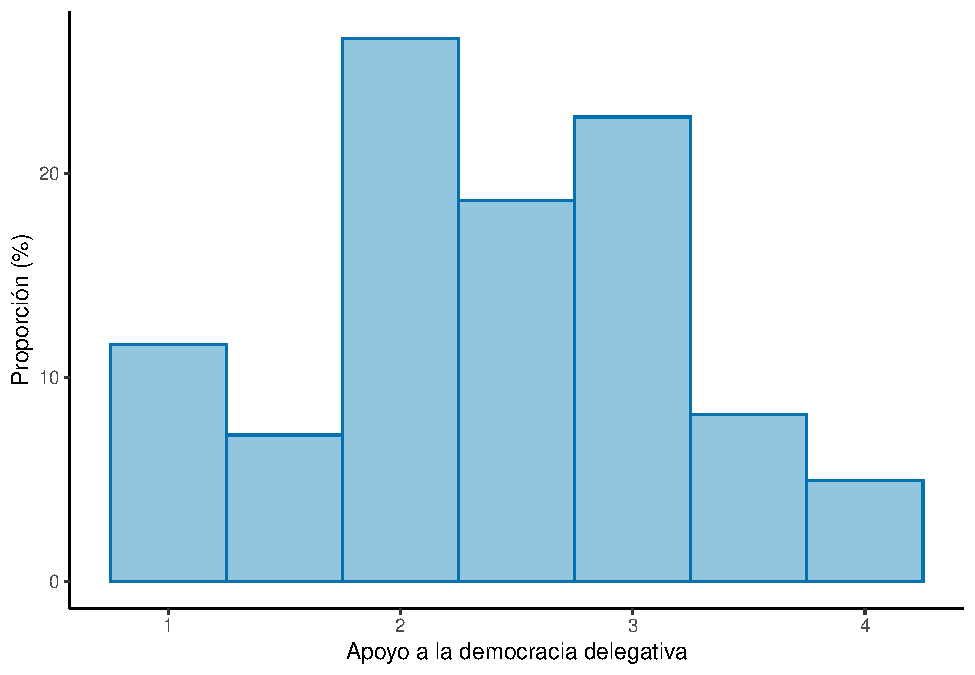
\includegraphics[width=1\linewidth,]{tesis_files/figure-latex/unnamed-chunk-7-1} 

}

\caption{Distribución Apoyo a Democracia Delegativa}\label{fig:unnamed-chunk-7}
\end{figure}
\FloatBarrier

Nota. Elaboración propia en base a datos de la Encuesta Mundial de Valores (Haerpfer et al., 2020).

Los grupos sociodemográficos que muestran un mayor respaldo a la democracia delegativa son las personas que se identifican políticamente de derecha (\(\bar{x}\)=2,66, \(s\)=0,99), con ingresos subjetivos medios-altos\footnote{En una escala del 1 al 10, se consideró como ingreso subjetivo bajo del 1 al 3; medio-baja del 4 al 5; medio-alto del 6 al 7; y alto del 8 al 10.} (\(\bar{x}\)=2,5, \(s\)=0,84), aquellas que se identifican como evangélicas (\(\bar{x}\)=2,48, \(s\)=0,84) o católicas (\(\bar{x}\)=2,44, \(s\)=0,78), las que no se identifican con ninguna posición política (\(\bar{x}\)=2,43, \(s\)=0,78), y las personas con edades comprendidas entre los 30 y los 44 años (\(\bar{x}\)=2,46, \(s\)=0,75). Por otro lado, en el extremo opuesto, se encuentran a las personas con ingresos subjetivos bajos (\(\bar{x}\)=2,22, \(s\)=0,81), sin afiliación religiosa (\(\bar{x}\)=2,24, \(s\)=0,83), aquellos políticamente identificados con la centro derecha (\(\bar{x}\)=2,3, \(s\)=0,99), los mayores de 60 años (\(\bar{x}\)=2,31, \(s\)=0,82), y las personas con ingresos subjetivos altos (\(\bar{x}\)=2,32).

\hypertarget{anuxe1lisis-de-clases-latentes-1}{%
\section{Análisis de Clases Latentes}\label{anuxe1lisis-de-clases-latentes-1}}

\hypertarget{anuxe1lisis-descriptivo-1}{%
\subsection*{Análisis Descriptivo}\label{anuxe1lisis-descriptivo-1}}
\addcontentsline{toc}{subsection}{Análisis Descriptivo}

\begin{figure}[!ht]

{\centering 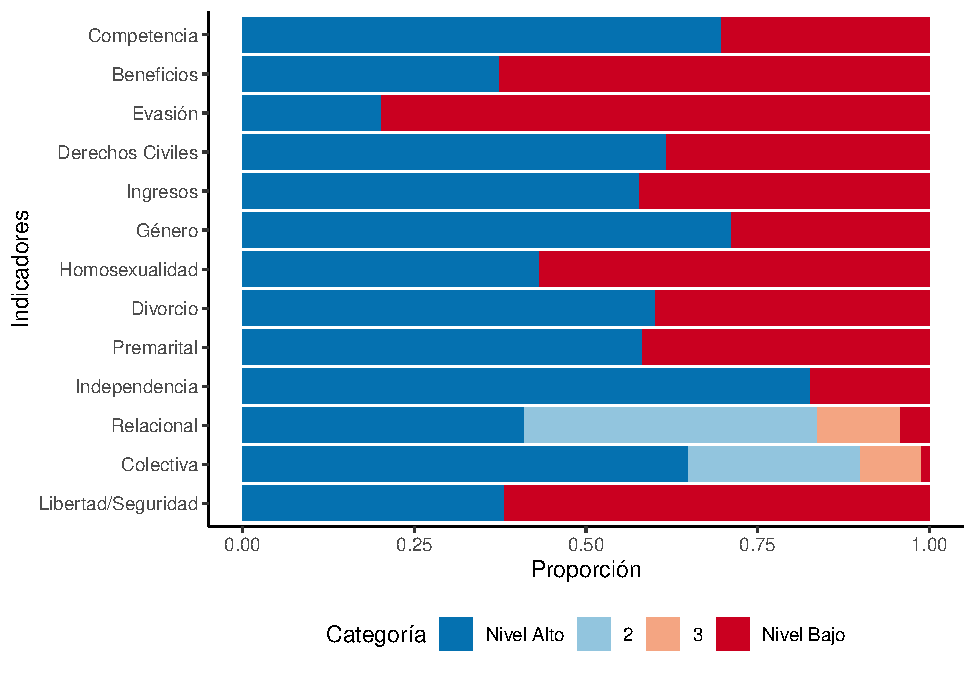
\includegraphics[width=1\linewidth,]{tesis_files/figure-latex/unnamed-chunk-8-1} 

}

\caption{Distribución indicadores de individualismo (recodificados)}\label{fig:unnamed-chunk-8}
\end{figure}
\FloatBarrier

Nota. Elaboración propia en base a datos de la Encuesta Mundial de Valores (Haerpfer et al., 2020); Todas las variables son dicotómicas, excepto los indicadores de independencia, interdependencia relacional e interdependencia colectiva, que no se recodificaron y se mantuvieron como variables categóricas de 4 categorías.

En la Figura 4.2 se presenta la distribución de los indicadores de individualismo para el total de la muestra. Se destaca una alta valoración de la competencia (70\%), pero un amplio rechazo al actuar estratégico cuando se trata de mentir para obtener beneficios sociales (63\%) o en la evasión en el transporte público (80\%). Además, se nota una valoración moderadamente alta de los indicadores de individualismo moral e individualismo expresivo.

El 83\% se siente a cargo de su vida, lo que refleja un alto nivel de independencia. De manera similar, un 84\% considera que hacer sentir orgullosos a sus padres es uno de los principales objetivos en sus vidas. Además, un 90\% de la población se siente cercana o muy cercana a su país. Estos hallazgos son coherentes con investigaciones previas que sugieren que las autoconcepciones independientes e interdependientes no son contradictorias, sino que muestran niveles igualmente altos en Chile \citep{benavides2020, kolstad2009}.

Por último, una proporción importante de la población (62\%) prioriza la seguridad (en rojo) por encima de la libertad (en azul). Este hallazgo -- que resulta interesante leerlo, además, a la luz de la crisis de seguridad que atraviesa el país actualmente -- podría representar evidencia a favor de que la autonomía no es el valor principal en base al cual las personas se constituyen como individuos en Chile \citep{martuccelli2010}.

\hypertarget{modelo-de-clases-latentes}{%
\subsection*{Modelo de Clases Latentes}\label{modelo-de-clases-latentes}}
\addcontentsline{toc}{subsection}{Modelo de Clases Latentes}

El siguiente paso, pues, es identificar si es posible identificar perfiles entre los que los indicadores seleccionados se comportan de manera diferenciada. Para llevar a cabo este análisis, se seleccionó un modelo de 4 clases en base a los estadísticos de ajuste que se muestran en la Figura 4.3, además de considerar criterios teóricos y de parsimonia \citep{collins2010}.

\begin{figure}[!ht]

{\centering 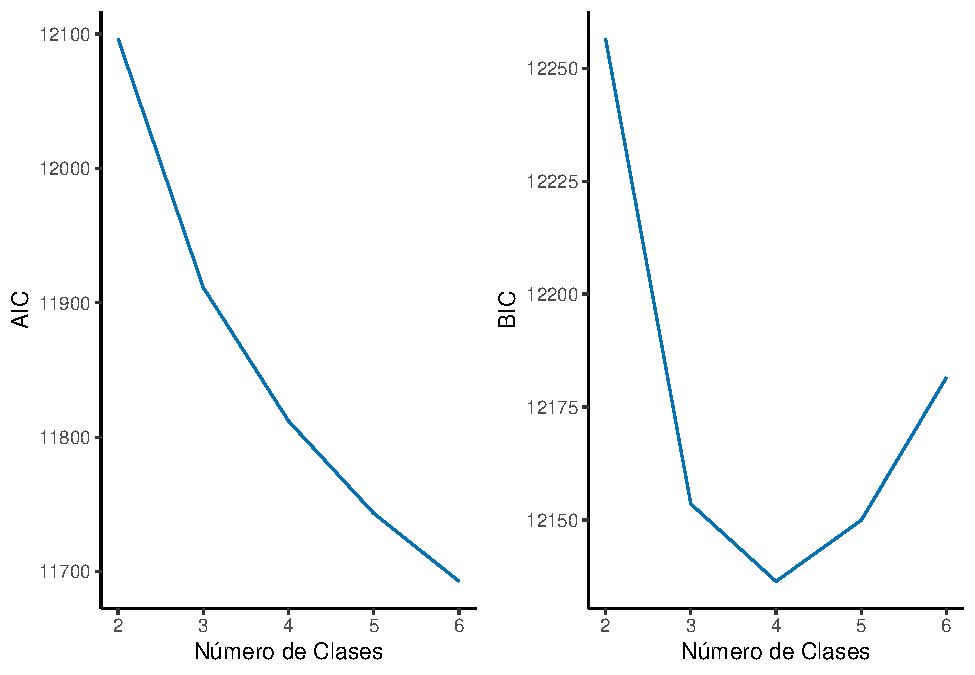
\includegraphics[width=1\linewidth,]{tesis_files/figure-latex/unnamed-chunk-9-1} 

}

\caption{Ajuste Estadístico de Modelos Estimados}\label{fig:unnamed-chunk-9}
\end{figure}
\FloatBarrier

Nota. Elaboración propia en base a datos de la Encuesta Mundial de Valores (Haerpfer et al., 2020).

Debido a las diferencias en las penalizaciones incorporadas en sus cálculos, cada indicador puede llevar a conclusiones diferentes: mientras que el BIC sugiere un modelo de 4 clases, el AIC apunta hacia uno de 6. Es importante señalar que se ha observado que el BIC puede predecir de manera más precisa el número de clases que el AIC, especialmente en muestras con más de 300 casos \citep{nylund2007}. Además, se deben tener en cuenta criterios sustantivos, como la parsimonia y la interpretabilidad teórica. Por ello, y luego de analizar las distintas configuraciones, se ha optado por el modelo de 4 clases, el cual se presenta a continuación en la Figura 4.4.

\begin{figure}[!ht]

{\centering 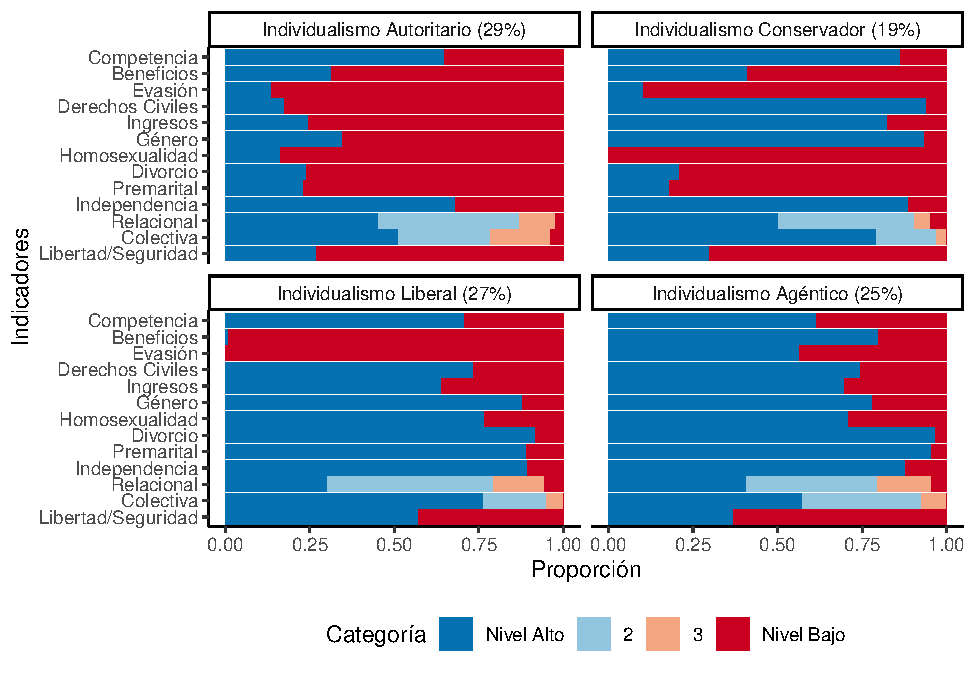
\includegraphics[width=1\linewidth,]{tesis_files/figure-latex/unnamed-chunk-10-1} 

}

\caption{Modelo de Clases Latentes de Individualismo (4 clases)}\label{fig:unnamed-chunk-10}
\end{figure}
\FloatBarrier

Nota. \(N\)=713; Parametros Estimados = 71; \(G^2\)= 3016,5 (df=642); \(AIC\)=11.812; \(BIC\)=12.136

Se observa que las cuatro clases muestran patrones distintos entre sí, así como diferencias respecto a la distribución promedio de la muestra. En la figura 4.5., se describe la distribución estimada de cada uno de los perfiles en la población.

\begin{figure}[!ht]

{\centering 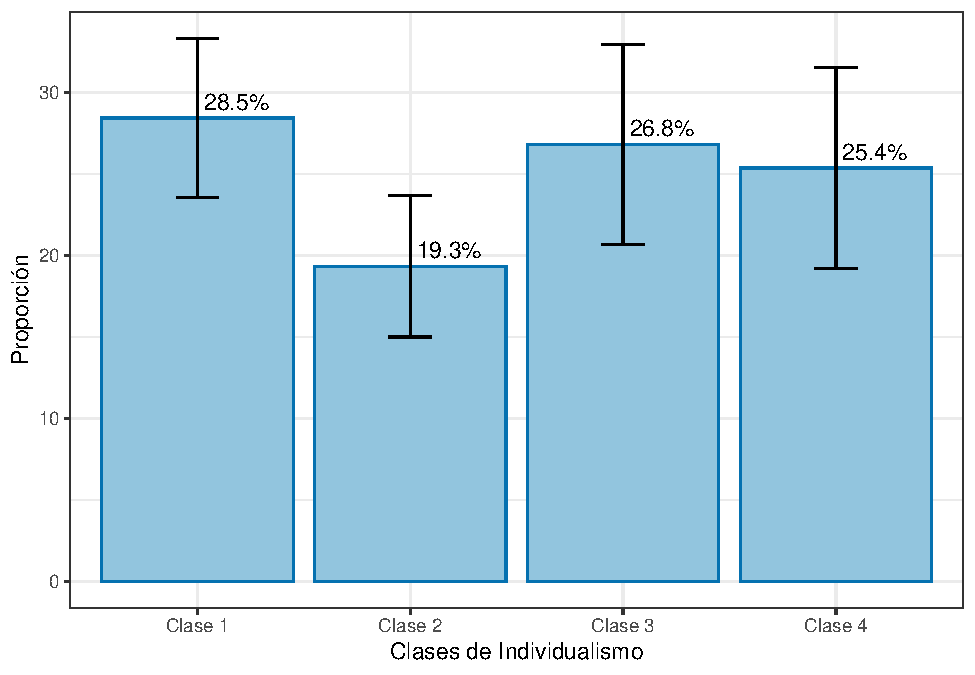
\includegraphics[width=1\linewidth,]{tesis_files/figure-latex/unnamed-chunk-11-1} 

}

\caption{Distribución estimada Clases Latentes}\label{fig:unnamed-chunk-11}
\end{figure}
\FloatBarrier

La clase 1 se caracteriza por valorar positivamente la competencia, pero a la vez tiende a rechazar la acción individual en diversas esferas. Por ejemplo, se observa un alto rechazo a evadir en el transporte público (88\%), una indiferencia hacia los derechos civiles (83\%), y un rechazo a la homosexualidad (84\%). Dicho en otras palabras, la acción individual cuenta con baja legitimidad tanto en la esfera económica, como en la política y en la expresiva. Para este grupo, de tal modo, la individualidad debe estar subsumida al respeto irrestricto a las normas sociales establecidas. Es posible que este deseo venga de una menor integración y de un mayor deseo por seguridad. Respecto a lo primero, es interesante destacar que esta clase presenta, además, el nivel más bajo de independencia (un igualmente alto 68\%) y de interdependencia colectiva (un 78\% se siente cercano o muy cercano al país). Asimismo, la probabilidad de que los miembros de esta clase prefieran la seguridad por sobre la libertad es la más alta entre las 4 clases, con un 73\%. Dado que la conformidad \citep{zakrisson2005} y la baja integración social \citep{gidron2020} son caracteristicas asociadas a las personalidades autoritarias, se ha decido bautizar a este perfil como \textbf{individualismo autoritario}

La edad promedio de este grupo es de 46,3 años, ligeramente superior al promedio de la muestra (44,3 años). Esta diferencia se debe principalmente a que solo el 14\% de las personas en este perfil tienen menos de 30 años \footnote{Un resumen detallado del cruce entre indicadores sociodemográficos y perfiles de individuo se presenta en los anexos.}. Además, es importante señalar que este grupo muestra un mayor nivel de religiosidad, al menos en términos nominales: el 67\% de sus miembros se identifica como católico, mientras que solo el 19\% no tiene afiliación religiosa. Un rasgo adicional interesante de este perfil es que presenta, al mismo tiempo, la mayor proporción de personas pertenecientes a la clase trabajadora (48\%) y de personas de la clase de servicios (26\%).

La clase 2 se caracteriza por una alta probabilidad de justificar la competencia y de legitimar el individualismo moral, mientras que rechaza tanto la acción estratégica como la individualidad en la esfera expresiva. Esto se ve reflejado en las altas probabilidades, mayores a la del resto de los grupos, de rechazar la homosexualidad (100\%), el divorcio (79\%) y el sexo premarital (82\%). Por otro lado, parece ser el grupo donde la interdependencia relacional cobra más importancia en las autoconcepciones de los individuos. Por último, la probabilidad de que los miembros de esta clase prefieran la seguridad por encima de la libertad es del 70\%.

Al igual que el individualismo autoritario, este grupo se caracteriza por tener una edad promedio superior al de la muestra (47,8 años promedio). Esto se refleja en que la proporción de personas menores de 30 en este perfil alcanza solo el 12\%, mientras que el 28\% tiene 60 años o más. En general, los individualistas conservadores se encuentran políticamente más a la centro derecha (36\%), son más católicos (63\%) que otros grupos y viven en ciudades más pequeñas (el 27\% vive en ciudades menores a 100.000 habitantes). También es el grupo que más reporta ingresos subjetivos altos (14\%, el doble del promedio de la muestra). Sin embargo, esto no se ve reflejado en el tipo de trabajos que realizan, pues la proporción de personas pertenecientes a la clase media y clase de servicios en este perfil se encuentran en torno al promedio de la muestra.

El lema ``Dios, Patria y Familia'' podría describir bien a este grupo. ¿Qué lo diferencia del individualismo autoritario? Principalmente su mayor compromiso con los valores del individualismo moral. Por ejemplo, la probabilidad de presentar una alta valoración de los derechos civiles alcanza un 73\%. Por estos motivos, se ha decido denominar a este perfil como un \textbf{individualismo conservador}

La clase 3 tiene algunos rasgos similares con el individualismo conservador. Por ejemplo, muestra una alta probabilidad de legitimar la competencia, y también el individualismo moral, además de rechazar de forma considerable las acciones estratégicas. Sin embargo, se distancia de sus pares conservadores en dos aspectos fundamentales: Por un lado, en la alta legitimidad del individualismo expresivo que se observa en este grupo. Por otro, en que es la única clase donde la probabilidad de elegir la libertad es mayor que la de preferir la seguridad. Se le ha denomidado como \textbf{individualismo liberal}, pues, sus valores parecen apuntar al respeto a la libertad y a la tolerancia de la acción individual en todas las esferas de la vida social, aunque manteniendo el respeto por algunas normas de convivencia. A pesar de que podría asemejarse al ``individualismo institucional'' descrito por Martuccelli \citeyearpar{martuccelli2010}, se diferencia de este por su marcado carácter relacional -- lo que parece ser un rasgo transversal a las cuatro clases de individualismo identificadas.

Por un lado, este grupo se destaca por una mayor proporción de personas en la izquierda y la centro izquierda del espectro político (28\%), pero también el que alberga la mayor cantidad de personas sin identificación política (29\%). Por otro lado, en contraste con las dos clases anteriores, este grupo se muestra como menos religioso, con un 36\% de sus miembros declarando no tener afiliación religiosa. Es el perfil con la menor cantidad de personas pertenecientes a la clase trabajadora (40\%), pero presenta la mayor proporción de individuos pertenecientes a las clases intermedias (37\%).

Finalmente, la clase 4 se caracteriza por legitimar la acción individual en todas las esferas, incluyendo (y de manera única en este sentido) las acciones estratégicas. Aunque muestra niveles menores de interdependencia colectiva en comparación con sus pares liberales y conservadores, los niveles de independencia en esta clase son más altos que los observados en el individualismo autoritario. La preferencia por la seguridad por sobre la libertad en este grupo alcanza un 63\%, en torno al promedio de la población. Siguiendo el trabajo de Araujo y Martuccelli \citeyearpar{araujo2012}, esto grupo enfatizaría la confianza depositada en sus propias habilidades, lo que los llevaría a legitimar en mayor medida acciones que transgreden normas sociales para obtener beneficios personales. Por esta razón, se ha decidido denominar a este perfil como \textbf{individualismo agéntico}

De los cuatro perfiles, este es el único en el que se observan diferencias en la composición de género, mostrando una leve feminización (56\%). Además, es un grupo más joven, con una edad promedio de 40,3 años. El 28\% de las personas en esta clase son menores de 30 años, mientras que solo el 9\% tiene 60 años o más. A pesar de que el 64\% vive fuera de la Región Metropolitana, se diferencia del ``individualismo conservador'' en que se concentra en ciudades con más de 100,000 habitantes: es menos un individualismo de capitales provinciales y más un individualismo de capitales regionales. Comparte con el individualismo liberal una baja identificación religiosa, ya que el 37\% de sus miembros declara no tener religión. Finalmente, es el grupo que menos reporta ingresos subjetivos altos (4\%), el que más lo hace en ingresos subjetivos medios-bajos (57\%), y el que tiene la menor proporción de personas en las clases de servicios (20\%).

Para cerrar esta sección, y con el fin de ilustrar los principales hallazgos obtenidos a partir del análisis de clases latentes, la figura 4.6. presenta un resumen gráfico de las principales caracteristícas de los perfiles identificados.

\begin{figure}[!ht]

{\centering 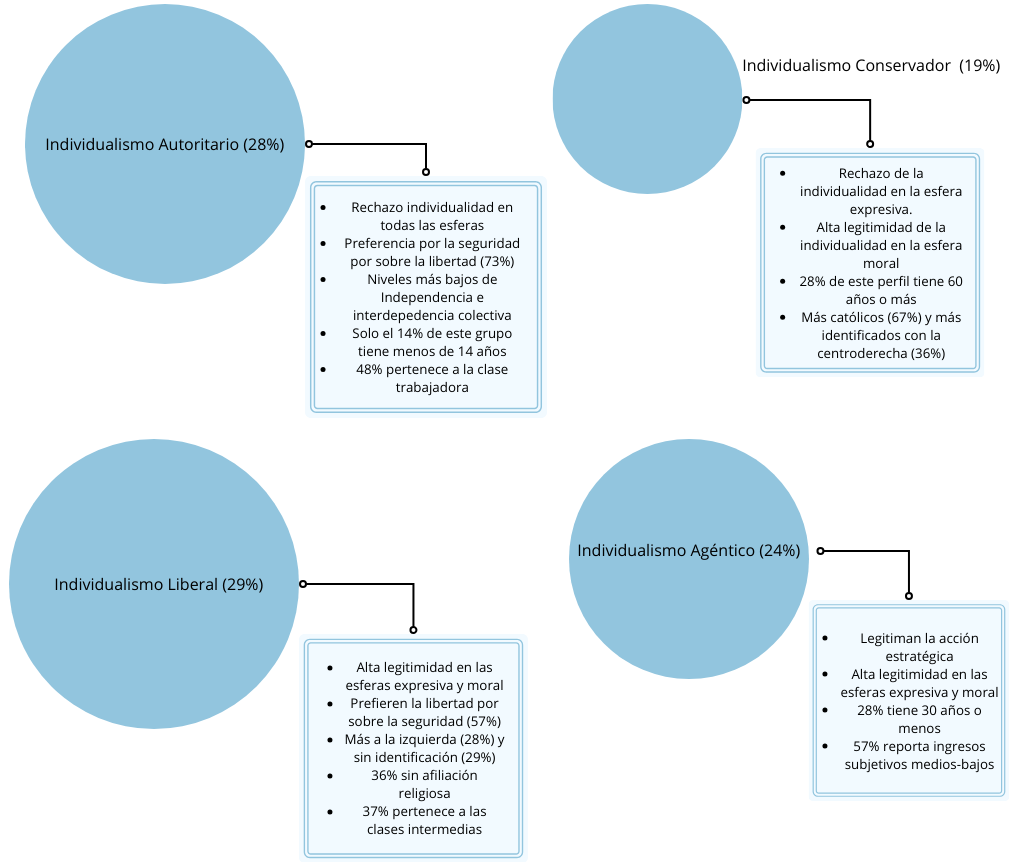
\includegraphics[width=1\linewidth,]{images/fig_esferas} 

}

\caption{Resumen Perfiles de Individualismo}\label{fig:nombre}
\end{figure}

\hypertarget{anuxe1lsis-de-varianza-y-modelos-de-regresiuxf3n}{%
\section{Análsis de Varianza y Modelos de Regresión}\label{anuxe1lsis-de-varianza-y-modelos-de-regresiuxf3n}}

En la Tabla 4.2, se presenta el promedio de apoyo a la democracia delegativa para cada perfil de individualismo identificado. Se puede observar que el grupo del Individualismo Agéntico muestra los mayores niveles de apoyo (\(\bar{x}\)=2,64, \(s\)=0,77), seguido por el Individualismo Autoritario (\(\bar{x}\)=2,58, \(s\)=0,68). En el extremo opuesto, se encuentra el Individualismo Conservador (\(\bar{x}\)=2,13, \(s\)=0,8), mientras que el Individualismo liberal se sitúa en torno al promedio.

\begin{table}[h]

\caption{\label{tab:unnamed-chunk-12}Promedio Apoyo a Democracia Delegativa por perfiles de individualismo}
\begin{tabular}[t]{>{\centering\arraybackslash}m{5.2cm}>{\centering\arraybackslash}m{2.8cm}>{\centering\arraybackslash}m{2.8cm}>{\centering\arraybackslash}m{2.8cm}}
\toprule
Perfiles & Apoyo a Lideres Fuertes & Apoyo a Expertos & Apoyo a Democracia Delegativa\\
\midrule
Individidualismo Autoritario & 2,56 & 2,58 & 2,58\\
Individualismo Conservador & 2,12 & 2,15 & 2,13\\
Individualismo Liberal & 2,33 & 2,38 & 2,35\\
Individualismo Agéntico & 2,56 & 2,69 & 2,64\\
\bottomrule
\end{tabular}
\end{table}
\FloatBarrier

Cabe destacar que la diferencia entre el Individualismo Agéntico y el Individualismo Autoritario se debe principalmente al apoyo a que los expertos tomen decisiones políticas. Así, mientras el apoyo a un liderazgo fuerte es idéntico en ambos perfiles (\(\bar{x}\)=2,56), el apoyo a los expertos es superior entre los miembros del Individualismo Agéntico (\(\bar{x}\)=2,69, \(s\)=0,86).

Como paso previo, se realizó un ANOVA para comprobar si existen diferencias significativas en las medias del apoyo a la democracia delegativa de los perfiles de individualismo. Los resultados apuntan a rechazar la hipótesis nula de que las medias de los grupos son iguales (\(F\)= 12,8; \(p\)\textless0,001). De tal modo, se procederá a estimar un modelo de regresión lineal que permita establecer si estas diferencias se mantienen una vez controladas por otras variables.

En la Tabla 4.3, se presentan los modelos estimados para predecir el apoyo a la democracia delegativa. En el Modelo 1, se incluye como único predictor el individualismo, que se ha convertido en una variable categórica a partir de las probabilidades posteriores estimadas por el modelo de Clases Latentes. Se especificó al Individualismo Conservador como variable de referencia, ya que esto permitiría apreciar mejor las diferencias entre grupos. De este modo, parece haber evidencia de una relación entre el individualismo y el apoyo a la democracia delegativa. En relación a ser un individualista conservador, ser un individualista autoritario (\(\beta\)= 0,44; \(p\)\textless0,001), un individualista agéntico (\(\beta\)= 0,30; \(p\)\textless0,001), o un individualista liberal (\(\beta\)= 0,21; \(p\)\textless0,05) está asociado con un efecto positivo y significativo en el apoyo a la democracia delegativa. En conjunto, el individualismo explicaría el 5\% de la varianza en el apoyo a la democracia delegativa.

\begin{table}[!h]

\caption{\label{tab:unnamed-chunk-13}Comparación Modelos de Regresión Lineal sobre el Apoyo a la Democracia Delegativa}
\centering
\begin{tabu} to \linewidth {>{\raggedright\arraybackslash}m{5cm}>{\centering}X>{\centering}X>{\centering}X}
\toprule
\multicolumn{1}{c}{ } & \multicolumn{3}{c}{Variable Dependiente: Apoyo a la Democracia Delegativa} \\
\cmidrule(l{3pt}r{3pt}){2-4}
  & (1) & (2) & (3)\\
\midrule
Constante & 2.134*** & 2.191*** & 1.802***\\
\addlinespace[0.3em]
\multicolumn{4}{l}{\textbf{Individualismo (1 = Conservador)}}\\
\hspace{1em}Autoritario & 0.442*** &  & 0.447***\\
\hspace{1em}Liberal & 0.212* &  & 0.175\\
\hspace{1em}Agéntico & 0.508*** &  & 0.504***\\
\addlinespace[0.3em]
\multicolumn{4}{l}{\textbf{Género (1 = Hombre)}}\\
\hspace{1em}Mujer &  & 0.085 & 0.083\\
Edad &  & -0.004 & -0.003\\
\addlinespace[0.3em]
\multicolumn{4}{l}{\textbf{Pos. Política (1 = Ninguna)}}\\
\hspace{1em}Izquierda &  & 0.053 & 0.023\\
\hspace{1em}Centro Izquierda &  & -0.127 & -0.115\\
\hspace{1em}Centro &  & -0.054 & -0.019\\
\hspace{1em}Centro Derecha &  & -0.320** & -0.256*\\
\hspace{1em}Derecha &  & 0.213 & 0.205\\
Ingresos Subjetivos &  & 0.057* & 0.057*\\
\addlinespace[0.3em]
\multicolumn{4}{l}{\textbf{Religión (1 = Ninguna)}}\\
\hspace{1em}Católica &  & 0.208** & 0.214**\\
\hspace{1em}Evangélica &  & 0.104 & 0.143\\
\hspace{1em}Otra &  & 0.291 & 0.269\\
\addlinespace[0.3em]
\multicolumn{4}{l}{\textbf{Tipo de Ciudad (1 = Santiago)}}\\
\hspace{1em}Rural &  & -0.313** & -0.297**\\
\hspace{1em}Menos de 100.000hab &  & -0.357*** & -0.307**\\
\hspace{1em}Más de 100.000hab &  & 0.013 & 0.045\\
\addlinespace[0.3em]
\multicolumn{4}{l}{\textbf{Clase Social (1 = de Servicios)}}\\
\hspace{1em}Clase Media &  & 0.183 & 0.181*\\
\hspace{1em}Clase Trabajadora &  & 0.294** & 0.267**\\
\midrule
$N$ & 623 & 533 & 533\\
$R^2$ & 0.059 & 0.091 & 0.151\\
$R^2$ Ajustado & 0.054 & 0.062 & 0.119\\
\bottomrule
\multicolumn{4}{l}{\rule{0pt}{1em}Nota. *:p<0,05; **:p<0.01; ***p<0.001}\\
\end{tabu}
\end{table}
\FloatBarrier

El Modelo 2 incluye únicamente las variables de control como predictoras. De esta manera, se observa que ni el género ni la edad muestran una relación significativa con el apoyo a la democracia delegativa. Sin embargo, vivir en zonas rurales (\(\beta\)= -0,31; \(p\)\textless0,01) o en ciudades de menos de 100,000 habitantes (\(\beta\)= -0,36; \(p\)\textless0,001), así como identificarse políticamente como de centro-derecha (\(\beta\)= -0,32; \(p\)\textless0,01) está asociado con un efecto negativo y significativo sobre el apoyo a la democracia delegativa. Por otro lado, el nivel de ingresos subjetivo (\(\beta\)= 0,06; \(p\)\textless0,05) y pertenecer a la clase trabajadora (\(\beta\)= 0,29; \(p\)\textless0,01) evidencian una relación positiva y significativa con el apoyo a la democracia delegativa. Este modelo explica el 6\% de la varianza en el apoyo a la democracia delegativa.

Finalmente, en el Modelo 3 se incluye tanto la variable categórica de individualismo como las variables de control. La principal diferencia respecto al Modelo 1 es que la asociación entre el apoyo a la democracia delegativa y el individualismo liberal, en relación al individualismo conservador, deja de ser significativa (\(\beta\)= -0,18, \(p\)=0,075). Posiblemente, esto se deba a su interacción con otras variables de control, particularmente con la identificación política.

Sin embargo, se mantiene la evidencia a favor de que, una vez controlado por las demás variables y en comparación con ser un individualista conservador, ser un individualista autoritario (\(\beta\)= 0,27, \(p\)\textless0,01), o un individualista agéntico (\(\beta\)= 0,33, \(p\)\textless0,001), está asociado positivamente al apoyo a la democracia delegativa. En total, este último modelo explica el 12\% de la varianza observada en el apoyo a la democracia delegativa.

Para comprender mejor cómo se comporta esta relación, se realizaron dos modelos de regresión logística, uno para cada indicador que compone el índice de apoyo a la democracia delegativa. Esto se hace con el propósito de establecer si las dimensiones del constructo se asocian de la misma manera con los perfiles de individualismo, o si se diferencias del índice en su conjunto. Se recodificaron las variables de modo que 0 representará un bajo apoyo y 1 un alto apoyo. En la Tabla 4.4, se resumen los resultados obtenidos

\begin{table}[!h]

\caption{\label{tab:unnamed-chunk-14}Modelos de Regresión Logística (Estimación de Odds Ratio)}
\centering
\begin{tabu} to \linewidth {>{\raggedright\arraybackslash}m{5cm}>{\centering}X>{\centering}X}
\toprule
  & Apoyo Líder Fuerte & Apoyo Expertos\\
\midrule
Constante & 0.169** & 0.158**\\
\addlinespace[0.3em]
\multicolumn{3}{l}{\textbf{Individualismo (1 = Conservador)}}\\
\hspace{1em}Autoritario & 3.161*** & 2.447**\\
\hspace{1em}Liberal & 1.564 & 1.390\\
\hspace{1em}Agéntico & 2.853*** & 4.795***\\
\addlinespace[0.3em]
\multicolumn{3}{l}{\textbf{Género (1 = Hombre)}}\\
\hspace{1em}Mujer & 1.437 & 1.075\\
Edad & 0.991 & 0.997\\
\addlinespace[0.3em]
\multicolumn{3}{l}{\textbf{Pos. Política (1 = Ninguna)}}\\
\hspace{1em}Izquierda & 1.265 & 1.576\\
\hspace{1em}Centro Izquierda & 1.094 & 0.764\\
\hspace{1em}Centro & 1.245 & 0.553*\\
\hspace{1em}Centro Derecha & 0.754 & 0.461*\\
\hspace{1em}Derecha & 2.890 & 2.169\\
Ingresos Subjetivos & 1.086 & 1.213**\\
\addlinespace[0.3em]
\multicolumn{3}{l}{\textbf{Religión (1 = Ninguna)}}\\
\hspace{1em}Católica & 1.693* & 1.735*\\
\hspace{1em}Evangélica & 1.635 & 2.194\\
\hspace{1em}Otra & 1.359 & 3.301**\\
\addlinespace[0.3em]
\multicolumn{3}{l}{\textbf{Tipo de Ciudad (1 = Santiago)}}\\
\hspace{1em}Rural & 0.624 & 0.532*\\
\hspace{1em}Menos de 100.000hab & 0.557* & 0.455**\\
\hspace{1em}Más de 100.000hab & 1.675* & 0.858\\
\addlinespace[0.3em]
\multicolumn{3}{l}{\textbf{Clase Social (1 = de Servicios)}}\\
\hspace{1em}Clase Media & 1.308 & 2.095**\\
\hspace{1em}Clase Trabajadora & 1.423 & 1.773*\\
\midrule
$N$ & 550 & 545\\
\bottomrule
\multicolumn{3}{l}{\rule{0pt}{1em}Nota. *:p<0,05; **:p<0.01; ***p<0.001}\\
\end{tabu}
\end{table}

Se observa que la asociación positiva entre el individualismo agéntico y el apoyo a la democracia delegativa se mantiene tanto para el apoyo a un líder fuerte (\(OR\)=2,9; \(p\)\textless0,001) como para el apoyo a expertos (\(OR\)=4,8; \(p\)\textless0,001). Lo mismo ocurre en el caso del individualismo autoritario (\(OR_{lider}\)=3,17; \(p\)\textless0,001. \(OR_{expertos}\)=2,45; \(p\)\textless0,01). Es interesante destacar que los \emph{odds ratios} para apoyo a un líder fuerte son superiores entre los individualistas autoritarios. Por el contrario, los \emph{odds ratios} para el apoyo a expertos son mayores en los individualistas agénticos.

Finalmente, aunque se mantiene la relación positiva con el individualismo liberal, nuevamente no es significativa ni para el apoyo a líderes fuertes (\(OR\)=0,45; \(p\)=0,12), ni para el apoyo a expertos (\(OR\)=0,33; \(p\)=0,25).

\hypertarget{discusiuxf3n}{%
\chapter{Discusión}\label{discusiuxf3n}}

\textbf{Apoyo a la Democracia Delegativa}

Se constató que el respaldo a la democracia delegativa en la sociedad chilena se sitúa en niveles intermedios, siendo el apoyo a que los expertos tomen decisiones para el país ligeramente más elevado que el respaldo a un líder fuerte. Es relevante señalar que se han identificado algunas disparidades entre grupos, siendo especialmente destacable el menor apoyo hacia la democracia delegativa entre quienes identifican con la centro-derecha, en contraposición a lo esperado a partir de la experiencia nacional \citep{navia2019} e internacional \citep{donovan2021}. Otro aspecto relevante de este dato es que se observan diferencias entre la centro-derecha y las posiciones más extremas de derecha, las cuales sí exhiben un respaldo superior a la democracia delegativa. Una posible explicación para esto podría radicar en diferencias de ingresos o de nivel educativo, lo que se traduciría en un menor respaldo a la democracia delegativa entre las personas con posiciones más moderadas de derecha \citep{kang2018}. Esto plantea hipótesis interesantes acerca de cómo el estatus socioeconómico puede interactuar o moderar el efecto de la posición política en el respaldo a la democracia.

Resulta llamativo, además, que las zonas rurales y las ciudades con menos de 100 mil habitantes sean las que menos respaldan la democracia delegativa, dado que la evidencia ha apuntado a que las áreas rurales suelen mostrar un mayor apoyo a candidatos de derecha populista en países como Estados Unidos \citep{schafft2021} o Alemania \citep{deppisch2022}. Este hallazgo merece una mayor atención en investigaciones futuras que se propongan trazar una geografía del autoritarismo en Chile y explorar cómo este fenómeno puede mostrar diferencias entre zonas urbanas y rurales.

\textbf{Perfiles de Individualismo}

El análisis de clases latentes realizado respalda la hipótesis de que los procesos de individualización divergen dentro de una misma sociedad. A partir de los datos examinados, se logró identificar cuatro perfiles distintos de individualismo en la sociedad chilena: individualismo autoritario, individualismo conservador, individualismo liberal e individualismo agéntico. Cada uno de estos perfiles equivale a variadas representaciones de la posición del individuo en la sociedad, y son resultado de combinaciones específicas de legitimidad de la acción individual en diferentes esferas, concepciones variadas del individuo, y diferentes valores e imperativos estructuralmente producidos. Además, la presencia de diferencias en edad, orientación política, ubicación geográfica o afiliación religiosa entre estos perfiles arroja luz sobre cómo los procesos estructurales interactúan de manera diferenciada con distintos segmentos de la población.

La tipología elaborada permite establecer un diálogo con la descripción del individualismo agéntico y el híper-actor relacional propuesto por Araujo y Martuccelli \citeyearpar{araujo2020}. Este modelo presenta dos características fundamentales: en primer lugar, la confianza depositada en las habilidades personales para afrontar la vida social, y en segundo lugar, la centralidad de las redes interpersonales. Se observó que una de las clases identificadas se acerca de manera más nítida a este modelo, de ahí que se haya decidido mantener la denominación de ``individualismo agéntico''. No obstante, se debe destacar que los otros perfiles también exhiben rasgos que hacen suponer que comparten, al menos parcialmente, la descripción de Araujo y Martuccelli.

En relación con la confianza en el esfuerzo y las habilidades personales, esto podría observarse en la alta valoración de la competencia y los elevados niveles de independencia observados de manera transversal en todos los perfiles. En términos generales, los datos sugieren que la mayoría de los chilenos cree poseer las habilidades necesarias para asumir el control de sus propias vidas.

Uno de los perfiles identificados, el individualismo agéntico, parece llevar este rasgo hasta el extremo, ya que es el único en el cual se legitima el actuar estratégico. Estar en un \emph{estado de alerta} para aprovechar las oportunidades es otra característica del individualismo agéntico descrita por Araujo y Martucceli \citeyearpar{araujo2014}. En la sociedad chilena, la capacidad de aprovechar las oportunidades suele ser vista como un motivo de orgullo personal, aunque no sin contradicciones, especialmente cuando se convierte en transgresión. Se podría pensar que esta tipología refleja esa tensión: Mientras tres de las clases identificadas parecen percibir el oportunismo como un vicio colectivo, el individualismo agéntico lo celebra como un virtud personal.

Por otro lado, el carácter relacional del individualismo chileno parece ser una característica que atraviesa todos los perfiles \citep{araujo2014}. Cierto es que se mide solo una identidad relacional (la familiar) y solo una identidad colectiva (la nacional). Pese a esto, no parece demasiado difícil argumentar la importancia de estas identidades y que incluirlas en el modelo sirve para un buen primer acercamiento.

También es importante señalar que el carácter relacional del individualismo chileno parece no entrar en contradicción con las concepciones independientes, que muestran niveles tan elevados como los indicadores de interdependencia. Esto es consistente tanto con las dos características que describen al individualismo agéntico \citep{araujo2020} como con las investigaciones sobre el \emph{self-construal} en Chile \citep{benavides2020, kolstad2009}. Además, ofrece más respaldo a la idea de que ubicar a Chile en un continuo entre el individualismo y el colectivismo resulta problemático. A pesar de que los chilenos mayoritariamente se identifican como individuos independientes, esto no se traduciría en la aceptación de ideales tipo \emph{self-made man}. Por el contrario, la evidencia parece apuntar a que el individualismo chileno, en todas sus variantes, no se comprende de manera aislada de las identidades familiares y nacionales de las personas.

En resumen, a partir de los datos analizados, se puede concluir que el individualismo agéntico representa el modelo predominante de individualismo en Chile. Sin embargo, el aporte de esta investigación radica en que, mediante el análisis de clases latentes, es posible observar cómo este modelo diverge dentro de la sociedad chilena. Para algunos, la acción individual debe estar subordinada al orden normativo, mientras que para otros es legítimo actuar de manera estratégica incluso si ello transgrede normas sociales. Mientras que para unos la individualidad tiene cabida en todas las esferas, para otros su legitimidad no alcanza para la esfera afectiva. De tal modo, este enfoque permite observar los matices y las divergencias de los procesos de individualización en Chile.

\textbf{Apoyo a la democracia delegativa y perfiles de individualismo}

El hecho de que haya sido posible establecer una relación estadísticamente significativa entre los perfiles de individualismo y el respaldo a la democracia delegativa debe ser considerado como una evidencia alentadora del potencial del modelo teórico de individualismo propuesto. Dos de los perfiles identificados muestran una asociación negativa con el apoyo a la democracia delegativa (el conservador y el liberal), mientras que los otros dos (el agéntico y el autoritario) presentan una relación positiva.

Cabe preguntarse si este no es un eje que permita distinguir entre los perfiles identificados: el individualismo conservador y el liberal podrían denominarse como \emph{individualismos cívicos}, orientados hacia lo público. En contraste, el autoritario y el agéntico podrían considerarse más bien \emph{hiperindividualismos}, que están orientados más bien hacia lo privado. En los primeros, la individualidad estaría vinculada a la pertenencia a una comunidad política; en los segundos, lo público representaría un desafío, un obstáculo que se debe evitar ya sea mediante la sumisión de la individualidad a un orden normativo (como en el caso del individualismo autoritario) o mediante la maximización de las habilidades personales (como es el caso del individualismo agéntico).

La afinidad entre estos tipos de individualismo y la democracia delegativa podría explicarse debido a que esta variante de democracia permite a los ciudadanos ejercer el voto periódicamente (rendición de cuentas vertical) para luego retirarse de la esfera pública hasta la próxima elección \citep{peruzzotti2008}. Pero esta apatía está lejos de ser un cheque en blanco: a la autoridad electa se le exigen resultados, incluso si ello implica transgredir la autonomía de otras instituciones del Estado (rendición de cuentas horizontal). Si la relación entre los hiperindividualismos y la democracia delegativa se explica por una mayor apatía hacia el espacio público, como aquí se plantea, se esperaría encontrar diferencias entre los perfiles de individualismo en variables como la participación política o la confianza generalizada.

Aunque la distinción entre individualismos cívicos e hiperindividualismos puede recordar los constructos de individualismo horizontal e individualismo vertical, respectivamente, es necesario realizar algunas precisiones. En primer lugar, cabe señalar que el individualismo horizontal pone énfasis, sobre todo, en la unicidad del individuo. Aunque esto podría describir a los individualistas liberales, se debe notar que los individualistas conservadores no parecen estar tan dispuestos a aceptar esa unicidad en la esfera expresiva. Por otro lado, aunque se puede inferir que los hiperindividualismos muestran componentes jerárquicos, también es posible observar rasgos de individualismo horizontal, especialmente en el individualismo agéntico, como en la alta legitimidad de la individualidad expresiva. Lo que distingue a los individualismos cívicos de los hiperindividualismos no son tanto las visiones jerárquicas o sobre la unicidad del individuo, sino más bien su posición frente a la esfera pública. Sin embargo, en futuras investigaciones se debería profundizar en la relación entre el modelo teórico propuesto aquí y otras mediciones de individualismo, incluyendo las escalas de individualismo vertical y horizontal.

Otro aspecto interesante que se debe destacar es que, mientras los individualistas autoritarios muestran un mayor respaldo a los líderes fuertes, los individualistas agénticos lo hacen a los expertos. Este hallazgo resulta relevante considerando que el individualismo agéntico, a diferencia del autoritario (pero en concordancia con el conservador y el liberal), exhibe altos niveles de apoyo a la individualidad en la esfera política. Esto podría indicar que lo que caracteriza al individualismo agéntico no sería tanto el autoritarismo, sino más bien una postura pragmática hacia la democracia. Este grupo podría valorar la democracia no necesariamente como un fin, sino como un medio que les permita resolver problemas privados.

\hypertarget{conclusiuxf3n}{%
\chapter{Conclusión}\label{conclusiuxf3n}}

Si bien los niveles de apoyo a la democracia delegativa son, en promedio, moderados, esta investigación permite concluir que existen diferencias significativas en tal apoyo entre los distintos perfiles de individualismo identificados: el autoritario, el conservador, el liberal y el agéntico. Además, se propuso que estos cuatro perfiles podrían distribuirse a lo largo de un eje que distingue entre individualismos cívicos e hiperindividualismos.

El individualismo conservador y el liberal, categorizados como individualismos cívicos, muestran menores niveles de apoyo a la democracia delegativa. Estos perfiles tienden a valorar la individualidad en conexión con la comunidad política, lo que se traduciría en un mayor apoyo a los ideales más represantivos de democracia.

Por otro lado, el individualismo autoritario y el agéntico, que pueden ser entendidos como formas de hiperindividualismo, presentan un nivel de apoyo superior a la democracia delegativa. Estos perfiles se inclinan por una actitud de apatía hacia la esfera pública, lo que sugiere una valoración de la democracia más como un medio para fines personales que como un fin en sí mismo.

En resumen, esta investigación sugiere que la relación entre el individualismo y el apoyo a la democracia delegativa es significativa, pero divergente entre distintos grupos. Mientras que los individualismos cívicos parecen valorar una visión más representativa de la democracia, los hiperindividualismos favorecen un enfoque más pragmático y apático hacia la esfera pública. Esto ilustra un panorama general en el que las manifestaciones del individualismo, y su relación con otros fenómenos, aparecen como más complejas de lo que otros estudios han propuesto.

\textbf{Alcances, limitaciones y reflexiones finales}

A continuación, se presentarán algunas reflexiones sobre las limitaciones y posibles líneas de investigación futuras que se desprenden de este estudio.

Para empezar, es importante reflexionar sobre las oportunidades que brinda el análisis de clases latentes en la investigación sobre los procesos de individualización en Chile. Dada la dificultad para traducir su marco teórico a una propuesta metodológica mediante las técnicas cuantitativas más comunes, la sociología del individuo se ha desarrollado principalmente desde una perspectiva cualitativa, resultando en descripciones profundas y estimulantes sobre el individuo en la sociedad chilena. Pese a ello, el enfoque metodológico adoptado en esta investigación permitió identificar algunos de los rasgos del individualismo agéntico descritos por Araujo y Martuccelli \citeyearpar{araujo2014}, al tiempo que ofrece una visión más matizada de cómo los procesos de individualización divergen en la sociedad chilena, diferenciándose entre grupos sociales y teniendo consecuencias en las actitudes políticas de los individuos.

Por supuesto, enfoques cualitativos y cuantitativos no deben ser vistos como competitivos, sino como complementarios en el desarrollo de una sociología del individuo. Las propias conclusiones aquí delineadas, y las hipótesis que de ellas se desprenden, se verían fuertemente enriquecidas si se incluyeran datos cualitativos que permitirían obtener una compresión más profunda de las distintas variantes de individualismo y su relación divergente con la esfera pública.

Ahora bien, es necesario reconocer las limitaciones que enfrentó esta investigación. La principal, posiblemente, se derive de los indicadores seleccionados. Aunque los resultados obtenidos parecen prometedores, es crucial continuar avanzando en la construcción y validación de indicadores que permitan traducir el modelo teórico aquí propuesto en un modelo de medición capaz de abordar el fenómeno del individualismo en Chile. En este sentido, hay cuatro puntos que vale la pena mencionar.

En primer lugar, es llamativo que no se observara una relación entre la valoración de la competencia y los indicadores de accionar estratégico, como evadir en el transporte público y mentir para obtener beneficios sociales. Se podría argumentar que estos representan dos dimensiones de un mismo constructo, el individualismo utilitario, con uno de ellos englobando la valoración de la competencia, el esfuerzo y la meritocracia, y el otro refiriéndose a los límites de esas conductas. Por ejemplo, una persona podría valorar la competencia entre individuos pero entender que ello implica el respeto común a ciertas normas; mientras que otros, como sería el caso de los individualistas agénticos, podrían percibir que la competencia justifica un \emph{todo vale}. Sin embargo, tampoco se puede descartar la posibilidad de que estos sean simplemente dos constructos diferentes. Sea cual sea el caso, es necesaria la elaboración y validación de indicadores que permitan medir el individualismo utilitario.

En segundo lugar, si los individualistas agénticos muestran una posición más pragmática frente a la democracia, ¿esto no debería reflejarse en una baja legitimidad del individualismo moral? El hecho de que los individualistas agénticos tengan una alta probabilidad de legitimar esa dimensión bien podría indicar que las razones para hacerlo no son necesaria o exclusivamente el individualismo. Otros factores, como la deseabilidad social, podrían estar sesgando estos resultados. Sin embargo, no es contradictorio que el individualismo agéntico legitime la individualidad en la esfera moral, especialmente si se vincula con los deseos de horizontalización del lazo social \citep{araujo2020a}. Preguntas que no aborden directamente la democracia, mediante temas tales como la pena de muerte o los derechos humanos, podrían mejorar la medición de este constructo.

En tercer lugar, como se ha mencionado anteriormente, hay razones para creer que la familia y la nación son particularmente relevantes a la hora de medir la interdependencia relacional y la identidad colectiva. No obstante, esto no significa que se deban descartar posibles diferencias en los perfiles identificados con respecto a otras identidades. Se podría hipotetizar, por ejemplo, que la identidad religiosa es más importante que la nacional entre los individualistas autoritarios, o que las amistades o las identidades profesionales pueden ser más relevantes, o bien complementar, la relevancia de la familia entre los individualistas liberales. Investigaciones futuras deberán abordar desde qué grupos de referencia los individuos construyen sus identidades.

Por último, la recodificación de variables continuas como dicotómicas es una solución pragmática, pero que no deja de ser problemática, ya que resulta en la pérdida de parte de la varianza de los ítems \citep{fernandes2019}. De tal modo, en el caso de construir indicadores originales a partir del modelo teórico de esta investigación, se debería considerar hacerlo directamente como variables categóricas que no necesiten recodificación para ser incluidas en el modelo de clases latentes. De esta manera, se obtendría claridad en los resultados sin sacrificar información ni poder estadístico.

Otras limitaciones provienen más bien de la muestra. Si 5 años ya se encuentra en el límite de lo que se puede considerar como datos relevantes para la actualidad, a esto se debe sumar que este último lustro ha sido uno particularmente tumultuoso: el Estallido Social, la Pandemia, el proceso constituyente, la crisis migratoria y la crisis de seguridad han sido algunos de los eventos de gran magnitud que han marcado la agenda durante los últimos años. ¿Están hoy los chilenos más dispuestos que hace 5 años a sacrificar su libertad y su individualidad en distintas esferas para obtener garantías de orden y seguridad? ¿Significó la emergencia sanitaria una transformación en como los expertos son percibidos y cuál debe ser su rol en la toma de decisiones? Entre las ollas comunes y los retiros de fondos previsionales, entre las protestas masivas y las cuarentenas, ¿cambiaron las concepciones -- independientes, relacionales y colectivas -- con las que los individuos construyen sus identidades? ¿Qué efectos puede tener la instauración del voto obligatorio en el eje individualismo cívico-hiperindividualismo, o en las percepciones de los ciudadanos sobre una democracia delegativa? Todas estas son preguntas relevantes que quedarán abiertas y deberán ser abordadas en el futuro.

Por otro lado, no se puede descartar la presencia de sesgos de deseabilidad social o por casos perdidos. La Encuesta Mundial de Valores es un extenso cuestionario que, con más de 300 preguntas, aborda temas que pueden resultar sensibles para muchas personas. No se puede descartar, por lo tanto, que ciertos grupos de la población estén moderando -- o incluso ocultando -- sus percepciones sobre temas políticos o valóricos. Se identificó que las personas mayores de 60 años, sin educación universitaria, sin identificación política y los habitantes fuera de Santiago muestran mayores probabilidades de no responder en las variables clave de este estudio. Frente a esto, una posibilidad a considerar es la imputación de datos para cubrir esta brecha.

A su vez, dado que Chile ha participado en 6 olas de la Encuesta Mundial de Valores desde 1990, se debería considerar correr los modelos aquí propuestos utilizando datos de ediciones anteriores (así como estar atento a la próxima versión a realizarse entre 2023 y 2026). Esto permitiría evaluar si los resultados obtenidos en este estudio guardan consistencia con el pasado, así como observar la evolución de estos indicadores a lo largo del tiempo.

Pese a estas limitaciones, el trabajo contenido en este documento logra obtener resultados relevantes. Se encontró evidencia de que distintas formas de individualismo pueden generar actitudes políticas diferentes respecto a la democracia, el tipo de liderazgos esperados y el rol que los expertos deben desempeñar en la sociedad. Es importante considerar que estas inclinaciones no surgen en un vacío, sino que son el resultado de la interacción de factores institucionales y estructurales con la agencia de los individuos. De esta manera, se espera que la lectura de esta investigación provoque la reflexión en torno a los tipos de individuos que nuestras instituciones, a través de sus programas e incentivos, contribuyen a producir, así como en las consecuencias de estos procesos para la democracia chilena y la vida social en general.

% %%%%%%%%%%%%%%%%%%%%%%%%%%%%%%%%%%%%%%%%%%%%%%%%%
% %%% Bibliography                              %%%
% %%%%%%%%%%%%%%%%%%%%%%%%%%%%%%%%%%%%%%%%%%%%%%%%%
%\addtocontents{toc}{\vspace{.9\baselineskip}}

\pagestyle{fancyplain}
\fancyhf{}
	 \fancyhead[RE]{\slshape Bibliografía}
	 \fancyfoot[C]{\thepage}
\phantomsection
\addcontentsline{toc}{chapter}{Bibliografía}
\bibliography{tesis}

%% All books from our library (SfS) are already in a BiBTeX file
%% (Assbib). You can use Assbib combined with your personal BiBTeX file:
%% \bibliography{Myreferences,Assbib}. Of course, this will only work on
%% the computers at SfS, unless you copy the Assbib file
%%  --> /u/sfs/bib/Assbib.bib


\hypertarget{Anexo}{%
\chapter*{Anexo}\label{Anexo}}
\addcontentsline{toc}{chapter}{Anexo}

\begin{table}[!h]

\caption{\label{tab:unnamed-chunk-14}Indicadores Sociodemográficos por Perfiles de Individualismo}
\fontsize{8}{10}\selectfont
\begin{tabu} to \linewidth {>{\raggedright}X>{\raggedleft}X>{\raggedleft}X>{\raggedleft}X>{\raggedleft}X}
\toprule
\multicolumn{1}{c}{Indicador} & \multicolumn{1}{c}{Autoritario} & \multicolumn{1}{c}{Conservador} & \multicolumn{1}{c}{Liberal} & \multicolumn{1}{c}{Agéntico}\\
\midrule
\addlinespace[0.3em]
\multicolumn{5}{l}{\textbf{Edad}}\\
\hspace{1em}30 a 44 & 34,00 & 34,59 & 36,27 & 33,73\\
\hspace{1em}45 a 59 & 30,00 & 27,07 & 28,43 & 28,99\\
\hspace{1em}Mayores de 60 & 21,50 & 26,32 & 15,69 & 9,47\\
\hspace{1em}Menores de 30 & 14,50 & 12,03 & 19,61 & 27,81\\
\addlinespace[0.3em]
\multicolumn{5}{l}{\textbf{Género}}\\
\hspace{1em}Hombre & 51,50 & 48,87 & 50,49 & 44,97\\
\hspace{1em}Mujer & 48,50 & 51,13 & 49,51 & 55,03\\
\addlinespace[0.3em]
\multicolumn{5}{l}{\textbf{Identificación Política}}\\
\hspace{1em}Ninguna & 24,00 & 16,54 & 28,92 & 23,08\\
\hspace{1em}Izquierda & 4,50 & 0,00 & 8,33 & 7,10\\
\hspace{1em}Centro Izquierda & 21,00 & 23,31 & 19,61 & 24,26\\
\hspace{1em}Centro & 28,00 & 24,81 & 23,53 & 21,30\\
\hspace{1em}Centro Derecha & 21,00 & 35,34 & 15,20 & 21,30\\
\hspace{1em}Derecha & 1,50 & 0,00 & 4,41 & 2,96\\
\addlinespace[0.3em]
\multicolumn{5}{l}{\textbf{Ingresos Subjetivos}}\\
\hspace{1em}Ingresos Altos & 7,00 & 13,53 & 4,41 & 4,14\\
\hspace{1em}Ingresos Bajos & 19,50 & 15,79 & 17,65 & 13,61\\
\hspace{1em}Ingresos Medios-Altos & 28,50 & 18,05 & 26,47 & 24,85\\
\hspace{1em}Ingresos Medios-Bajos & 45,00 & 52,63 & 51,47 & 57,40\\
\addlinespace[0.3em]
\multicolumn{5}{l}{\textbf{Religion}}\\
\hspace{1em}Sin religión & 19,07 & 21,21 & 35,18 & 36,42\\
\hspace{1em}Católica & 67,01 & 62,88 & 55,28 & 53,70\\
\hspace{1em}Evangélica & 7,22 & 8,33 & 6,03 & 4,94\\
\hspace{1em}Otra & 6,70 & 7,58 & 3,52 & 4,94\\
\addlinespace[0.3em]
\multicolumn{5}{l}{\textbf{Tipo de Ciudad}}\\
\hspace{1em}Santiago & 44,00 & 28,57 & 38,73 & 36,09\\
\hspace{1em}Rural & 13,50 & 9,77 & 13,24 & 13,02\\
\hspace{1em}Menos de 100.000 & 17,00 & 26,32 & 11,76 & 14,20\\
\hspace{1em}Sobre 100.000 & 25,50 & 35,34 & 36,27 & 36,69\\
\addlinespace[0.3em]
\multicolumn{5}{l}{\textbf{Clase Social}}\\
\hspace{1em}Clase de Servicio & 26,16 & 23,93 & 23,30 & 20,67\\
\hspace{1em}Clase Media & 26,16 & 34,19 & 36,93 & 37,33\\
\hspace{1em}Clase Trabajadora & 47,67 & 41,88 & 39,77 & 42,00\\
\bottomrule
\multicolumn{5}{l}{\rule{0pt}{1em}\textit{Nota.} Porcentajes son relativos al total de las columnas}\\
\end{tabu}
\end{table}

\end{document}
